%\cleardoublepage
\clearpage
\section{情绪诱发方案与实验数据采集}
对于情绪诱发范式,论文选用研究中较为常用的电影片段诱发方式,可操作性强且诱发效果好。
考虑到视频片段的情绪诱发效果受个体差异影响较大,同时还受到国内外文化差异的影响,在情绪生理唤醒实验前设置情绪刺激材料的评价实验,以挑选诱发效果更好的电影片段。
以下介绍完整的实验方案和数据采集过程,本实验已通过浙江大学心理与行为科学系医学伦理委员会的科研项目伦理审查(浙大心理申伦[2022]059号)。

\subsection{情绪刺激材料评价实验}
\subsubsection{视频选取}

电影片段的选取主要参考DECAF数据库\cite{DECAF2015},分别选取了4个恐惧视频片段和9个愉悦视频片段进行实验,视频信息汇总如\autoref{tab:Film-to-choose}所示。
\begin{table}[htbp]
    \centering
    \footnotesize
    \setlength{\abovecaptionskip}{0.1cm}
    \setlength{\belowcaptionskip}{0.2cm}
    \renewcommand\arraystretch{1.5}
    \caption[电影片段汇总表]{电影片段汇总表}
    \label{tab:Film-to-choose}
    \setlength{\tabcolsep}{0.25cm}{
        \begin{tabular}{ccccl}
            \toprule
            \textbf{目标情绪}       & \textbf{视频序号} & \textbf{片段名称} & \textbf{片段时长(min:sec)} & \textbf{视频剧情概要}                                                               \\ \midrule
            \multirow{4}{*}{恐惧} & 1             & 《闪灵》          & 1:18          & 孩子走进酒店房间找妈妈                                                              \\
                                & 2             & 《黑天鹅》         & 1:02          & 女士注意到她周围的超自然活动                                                           \\
                                & 3             & 《惊魂记》         & 1:15          & 女士在浴缸中被闯入者杀死                                                             \\
                                & 4             & 《午夜凶铃》        & 2:48          & \begin{tabular}[c]{@{}l@{}}男人的电视自动打开,一个女孩爬了出来\\ 并把头发从脸上扯了下来\end{tabular} \\ \midrule
            \multirow{9}{*}{愉悦} & 1             & 《飞屋环游记》       & 1:07          & 害羞、安静的男孩Carl遇到了精力充沛的Elle                                                 \\
                                & 2             & 《八月迷情》        & 1:29          & 儿子在音乐会表演时遇到了他失去的母亲                                                       \\
                                & 3             & 《楚门的世界》       & 1:00          & Truman和爱人去海滩度过了一个浪漫的夜晚                                                   \\
                                & 4             & 《机器人总动员》      & 1:33          & Wall-E和Eve在一起度过了一个浪漫的夜晚                                                  \\
                                & 5             & 《真爱至上》        & 0:51          & 爱无处不在的叙事                                                                 \\
                                & 6             & 《光辉岁月》        & 0:52          & Titans赢得了足球比赛                                                            \\
                                & 7             & 《美丽人生》        & 0:56          & 滑稽的Guido假扮成教育官员来到一所学校                                                    \\
                                & 8             & 《贫民窟的百万富翁》    & 1:20          & Latika和Jamal在火车站会合                                                       \\
                                & 9             & 《十面埋伏》        & 1:16          & 年轻的武士用花束迎接他的爱人                                                          \\ \midrule
            \multirow{2}{*}{平静}  & 1 & 《傲慢与偏见》 & 1:36 & 女士在房屋周围散步      \\          
                                 & 2             & 《王者之旅》        & 3:11          & 男士发现他的儿子会下国际象棋并和他下了一盘                                                       \\ \midrule
            练习视频 & 1 & 进度条动画 & 0:05 &  /   \\ \bottomrule
             \end{tabular}}
\end{table}

\subsubsection{实验流程}
% \raggedbottem
被试进入实验后,首先登记被试的身份信息(编号、姓名、性别、年龄),同时由主试阐述研究背景、实验过程和可能出现的不适。
没有疑问后,被试签署知情同意书(详细内容见附录),观看指导语视频,视频详细介绍了整个实验流程和被试需要进行的操作。
指导语视频完成后,实验正式开始,具体流程如下:

(1)	被试在程序首页填写人口学信息(性别、年龄)和组别(由主试告知)后,进入视频播放界面;

(2)	首先观看练习视频,再观看其余情绪视频(视频以伪随机顺序播放,以保证相同类别不会连续呈现)。

(3)	每一段视频结束后,被试对视频诱发的情绪做出主观评价,包括自我评估量表(唤醒度、效价、支配度,如\autoref{fig:Program-1}所示;喜好程度、熟悉程度;是否有回避行为)和情绪评价量表(快乐、悲伤、愤怒、恐惧,9点文字量表)
\vspace{-1ex}
\begin{figure}[htbp]
    \centering
    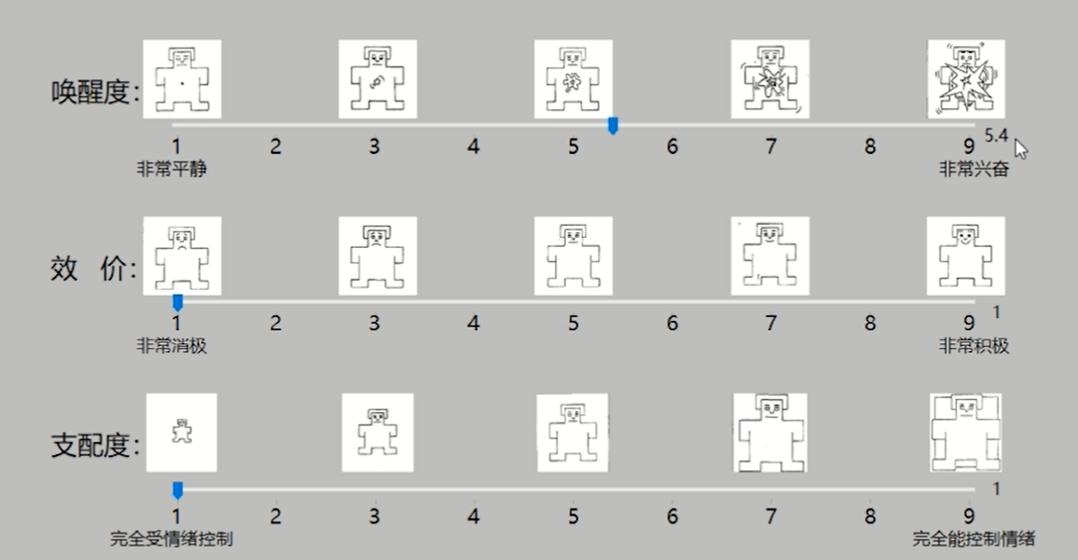
\includegraphics[width=\linewidth]{Program-1.png}
    \caption[自我评估量表示意图]{自我评估量表示意图}{\label{fig:Program-1}}
\end{figure}
\vspace{-3ex}

(4)	每一段视频的自我评价后,被试需要正确计算两道计算题后休息30s以恢复平静状态和消除上一个电影片段对下一个电影片段的影响。

(5)	观看完成所有视频后,被试完成抑郁PHQ-9、焦虑GAD-7量表,结束实验。


\subsubsection{情绪诱发材料分析结果}
情绪刺激材料评价实验共征集到66名被试,每个电影片段至少有33位被试观看且性别比例均衡,满足心理学实验30人大样本的要求,可以认为在此基础上筛选出的视频材料具有情绪诱发上的普适性。
以下介绍视频片段的筛选步骤,包括成功指数计算和唤醒度效价检验,以选出能成功诱发目标情绪且诱发效果较好的视频片段。

(1)成功指数计算

成功指数,即Z(情绪命中率)+Z(情绪强度),是衡量目标情绪是否被成功单独诱发的评价指标,
其中情绪命中率指对目标情绪的评分比所有非目标情绪至少都高一分的被试比例,情绪强度指目标情绪的平均分数。
根据实验数据计算成功指标如\autoref{tab:Success-index}所示。
\begin{table}[htbp]
    \centering
    \footnotesize
    \setlength{\abovecaptionskip}{0.1cm}
    \setlength{\belowcaptionskip}{0.2cm}
    \renewcommand\arraystretch{1.5}
    \caption[视频片段成功指数计算结果]{视频片段成功指数计算结果}
    \label{tab:Success-index}
    \setlength{\tabcolsep}{0.5cm}{
        \begin{tabular}{cccclc}
            \toprule
            \textbf{目标情绪}       & \textbf{视频序号} & \textbf{命中率} & \textbf{恐惧程度} & \textbf{快乐程度} & \textbf{成功指数} \\ \midrule
\multirow{4}{*}{恐惧} & 1             & 87.88\%       & 5.92          & 1.88   &-0.18       \\
                    & 2             & 91.43\%       & 7.24          & 1.19     &2.60     \\
                    & 3             & 64.86\%       & 5.99          & 1.36     &-2.22     \\
                    & 4             & 74.29\%       & 6.66          & 1.92      &-0.09    \\ \midrule
\multirow{9}{*}{愉悦} & 1             & 97.06\%       & 1.19          & 6.56   &3.16       \\ 
                    & 2             & 94.59\%       & 1.03          & 5.22     &0.10     \\
                    & 3             & 89.19\%       & 1.15          & 5.61    &-0.23      \\
                    & 4             & 97.14\%       & 1.25          & 6.54    &3.15      \\
                    & 5             & 85.29\%       & 1.04          & 5.54    &-1.16      \\
                    & 6             & 91.43\%       & 1.21          & 5.03    &-0.90      \\
                    & 7             & 85.71\%       & 1.02          & 5.22    &-1.67      \\
                    & 8             & 82.35\%       & 1.07          & 5.44   &-1.93       \\
                    & 9             & 89.19\%       & 1.01          & 5.48   &-0.48      \\ \midrule
                    \multirow{2}{*}{平静}  & 1 & / & 1.05 & 5.46   &/   \\          
                    & 2             & /        & 1.06          &   3.82   &/    \\ \bottomrule            
            \end{tabular}}
\end{table}

分析上表发现,恐惧片段1、2和4以及愉悦片段1、3和4的成功指数相对较高,但考虑到恐惧片段4的情绪命中率相对较低,所以不纳入选择。
平静片段1的快乐程度过高,也不纳入选择。

(2)唤醒度效价检验

唤醒度和效价是情绪维度模型(Russell环形模型\cite{Russell1980})中的两个重要维度,能够将不同的情绪区分在模型的不同象限,
其中唤醒度表征情绪是偏向平静无聊或是兴奋紧张的程度,效价则表征情绪消极或积极程度。
视频片段的唤醒度和效价评分汇总如\autoref{tab:V-A}所示。
% \vspace{-4ex}

\begin{table}[htbp]
    \centering
    \footnotesize
    \setlength{\abovecaptionskip}{0.1cm}
    \setlength{\belowcaptionskip}{0.2cm}
    \renewcommand\arraystretch{1.5}
    \caption[视频唤醒度效价检验结果]{视频唤醒度效价检验结果}
    \label{tab:V-A}
    \setlength{\tabcolsep}{0.7cm}{
        \begin{tabular}{cccc}
            \toprule
            \textbf{目标情绪}       & \textbf{视频序号} & \textbf{唤醒度} & \textbf{效价} \\ \midrule
            \multirow{4}{*}{恐惧} & 1             & 6.85         & 3.59        \\
                                & 2             & 7.91         & 2.13        \\
                                & 3             & 6.93         & 2.70        \\
                                & 4             & 7.39         & 2.80        \\ \midrule
            \multirow{9}{*}{愉悦} & 1             & 5.99         & 6.87        \\ 
                                & 2             & 4.60         & 6.30        \\
                                & 3             & 5.55         & 6.43        \\
                                & 4             & 5.53         & 7.26        \\
                                & 5             & 4.94         & 7.03        \\
                                & 6             & 5.27         & 6.56        \\
                                & 7             & 4.86         & 6.37        \\
                                & 8             & 5.10         & 6.04        \\
                                & 9             & 4.98         & 6.50        \\ \bottomrule
            \end{tabular}}
\end{table}
\vspace{-2ex}

在\autoref{tab:V-A}的基础上计算每个视频片段唤醒度(A)和效价(V)的均值(Mean)和标准差(STD),
并做一定的数学处理以消除维度影响,将V-A二维空间的中心转移到绝对中性点(5,5),处理公式如下:
\vspace{1ex}
\begin{equation}
    \label{equ:Mean}
    \text{A/V}= \frac{(\text{Mean}-5)}{\text{STD}}
    % \vspace{-8ex}
\end{equation}

根据重新计算得到的唤醒度和效价绘制V-A二维图(如\autoref{fig:V-A}),以检验视频片段诱发情绪的有效性。  
\begin{figure}[htbp]
    \centering
    \vspace{-0.2em}
    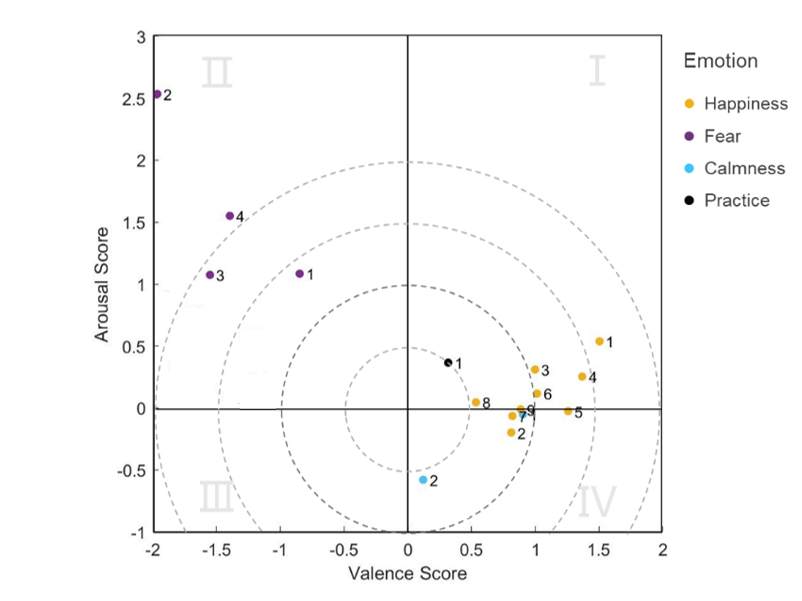
\includegraphics[width=.7\linewidth]{V-A.png}
    % \setlength{\abovecaptionskip}{0.2em}
    \caption[视频唤醒度效价分布图]{视频唤醒度效价分布图}{\label{fig:V-A}}
\end{figure}

分析\autoref{fig:V-A}发现,恐惧片段1、2和愉悦片段1、3、4在V-A二维图中的分布与理论相符,且与中性情绪点之间的距离较远,能够有效诱发被试的情绪。
同时,平静片段2的效价趋于中性点,唤醒度也相对较小,能够有效诱发被试的平静状态。

综上,根据成功指数的筛选和唤醒度效价的检验,最终选择恐怖片段《闪灵》《黑天鹅》、愉悦片段《飞屋环游记》《楚门的世界》《机器人总动员》
和平静片段《王者之旅》作为情绪唤醒生理实验的视频材料。

\subsection{情绪唤醒生理实验}
通过情绪刺激材料评价实验,本研究筛选出了能够成功诱发恐惧、愉悦情绪且诱发效果较好的普适性视频材料。
在此基础上进行情绪唤醒生理实验的被试,均可以认为被成功诱发目标情绪。下面介绍生理实验的信号采集设备和实验流程。

\subsubsection{实验设备}

本研究使用迈瑞ePM 12M生理信号监护仪采集心电、脉搏波和呼吸信号,采样率分别为500Hz,125Hz和60Hz。监护仪配置的移动模块(EP20)外观如\autoref{fig:new-ePM15}所示。
\begin{figure}[htbp]
    \centering
    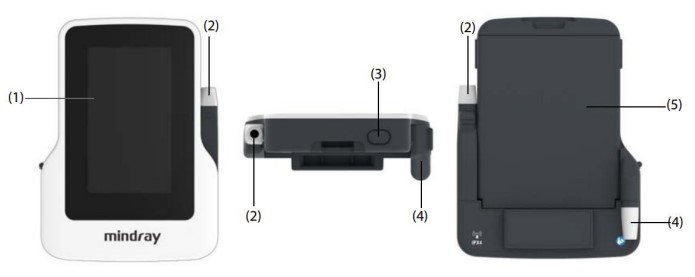
\includegraphics[width=.75\linewidth]{ePM15.jpg}
    \caption[迈瑞ePM 12M生理信号监护仪EP20模块外观]{迈瑞ePM 12M生理信号监护仪EP20模块外观}{\label{fig:new-ePM15}}
\end{figure}

其中(1)为显示屏,(2)为心电信号传感器的电缆线接口,(3)为开/关机键,(4)为脉搏波传感器的电缆线接口,(5)为电池仓。实验中EP20通过腕带固定在被试的左手手腕,
采集和分析心电和脉搏波等信号并将数据以无线方式发送至监护仪。

实验过程中,心电信号采用三导联电极进行采集,脉搏信号采用透射式血氧探头进行采集,呼吸信号由监护仪使用阻抗法从心电信号中自动提取得到,佩戴方式分别如\autoref{fig:new-ECGelctrode}和\autoref{fig:new-fingerelectrode}所示。

\begin{figure}[htbp]
    \hspace {0.4cm}
    \centering
    \begin{minipage}[l]{0.30\textwidth}
        % \hspace {-1cm}
        \centering
        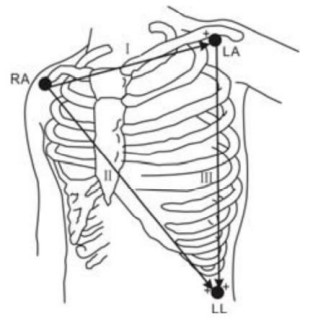
\includegraphics[width=0.9\textwidth]{ECGelctrode.jpg}
        \caption[心电电极安装示意图]{心电电极安装示意图}
        \label{fig:new-ECGelctrode}
    \end{minipage}
    \hspace{.65in}
    \begin{minipage}[c]{0.4\textwidth}
        \hspace {-1cm}
        \centering
        \vspace{-1.5em}
        \setlength{\abovecaptionskip}{3em}
        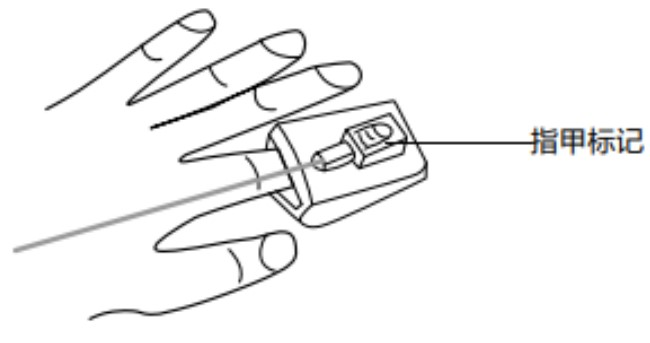
\includegraphics[width=\textwidth]{fingerelectrode.jpg}
        \caption[指夹佩戴示意图]{指夹佩戴示意图$\qquad$ $\qquad$ $\quad$ }
        \label{fig:new-fingerelectrode}
    \end{minipage}
\end{figure}

其中RA(右上电极)贴在胸骨右缘锁骨中线第一肋间,LA(左上电极)贴在胸骨左缘锁骨中线第一肋间,LL(左下电极)贴在左锁骨中线剑突水平处。
贴电极片前使用生理盐水棉球或酒精棉片擦拭被试相应位置的皮肤,去除油性残渣及死皮细胞,并避开出血或破损的皮肤。
脉搏波信号的测量部位一般为食指指尖,若食指出现损伤,可换成中指或其他手指佩戴。佩戴时把手指放入指套内部,
使指甲与传感器表面的指甲标记位置对应,指尖触及但不超出指套顶端,确保发光管发出的所有光线能够全部通过被试组织。

% 实验时将EP20的腕带安放在被试的左手手腕,调整腕带长度并粘紧魔术贴,确保仪器位置固定但不会压迫被试的手腕。整体连接方式如\autoref{fig:new-allelectrode}所示,其中(1)为血氧传感器,(2)为腕带,(3)为EP20,(4)为ECGcable,(5)为心电电极。
% \begin{figure}[htbp]
%     \centering
%     \vspace{-0.2em}
%     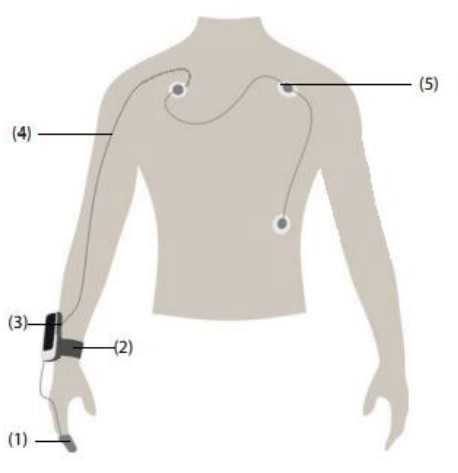
\includegraphics[width=.35\linewidth]{allelectrode.jpg}
%     \setlength{\abovecaptionskip}{0.2em}
%     \caption[信号采集仪器佩戴示意图]{信号采集仪器佩戴示意图}{\label{fig:new-allelectrode}}
% \end{figure}

\subsubsection{实验流程}
被试完成信息登记、知情同意书签署后,由主试协助佩戴实验装置,主要包括采集心电的三导联电极(LL、LA、RA)和佩戴在被试左手食指的指夹。被试被要求在实验正式开始前调整座位,保证在实验过程中身体姿态和左手的稳定。
观看完成指导语视频后,实验正式开始,流程与情绪刺激材料评价实验相同,此处不再赘述。

\clearpage
\section{信号预处理与特征提取}
情绪诱发实验共收集到66位被试的生理数据。本研究首先对采集得到的外周生理信号进行质量分析和时间校准,删去质量不佳的部分数据,并对其余有效的生理信号进行合理分段,
然后以片段为单位对生理信号进行预处理。最后,从时域、频域和非线性三个维度提取情绪识别的潜在有效特征以进行后续统计学分析和分类模型构建。

\subsection{数据清洗}
由于仪器内部时间与标准北京时间的误差,导出生理数据后首先需要将仪器记录的时间信息与实验程序记录的时间信息进行校准,从头部或尾部对齐信号。

整合被试的反馈信息发现,情绪诱发实验中容易出现因为专注于观看电影片段而忘记按键或不同程度延迟按键的情况,同时考虑到使用视频的时长较短
(一到三分钟),最终对被试观看电影片段时的生理信号采用每20s截取为一段数据的分段方式。分段完成后,使用图形界面查看每段数据的波形,筛选出心电、
脉搏和呼吸信号均有效的数据文件并在此基础上筛选出恐惧、愉悦和平静状态均至少包含一段有效生理数据的有效被试。

% 清洗完成情绪唤醒生理实验的66份被试数据后,共获得41位有效被试总计328段平静片段、102段恐惧片段和324段愉悦片段的有效数据。剩余被试数据未采用的主要原因为:
% (1)设备原因导致有较多被试呼吸信息大范围失真;(2)部分被试参加过情绪刺激材料评价实验后参加情绪唤醒生理实验,因观看视频基本相同,判为重复不采用;
% (3)极少数被试因不明原因出现数据异常、丢失的情况。

清洗完成情绪唤醒生理实验的66份被试数据后,发现部分数据存在以下问题:
(1)设备原因导致有较多被试呼吸信息大范围失真;(2)部分被试参加过情绪刺激材料评价实验后参加情绪唤醒生理实验,因观看视频基本相同,判为重复不采用;
(3)极少数被试因不明原因出现数据异常、丢失的情况。
最终,心电信号有效的被试数据为66份,心电和脉搏波信号都有效的为55份,心电、脉搏波和呼吸信号均有效的为41份。
因后续还需提取大量的呼吸特征,研究选用了41位三个生理信号均有效的被试数据,获得了328段平静片段、102段恐惧片段和324段愉悦片段的有效数据。

\subsection{信号预处理}
\subsubsection{心电信号预处理}
心电信号的预处理包括以下四个步骤:

(1)去噪

心电信号的频率范围为0.05$ \sim $100Hz,主要能量集中在5$ \sim $20Hz,采集过程中的主要噪声包括基线漂移(0.05$ \sim $2Hz)、工频干扰(50Hz)和肌电干扰
(5$ \sim $2000Hz,主要能量集中在30$ \sim $300Hz)等。本次实验采用的设备(迈瑞ePM 12M生理信号监护仪)内置部分滤波算法,故后续仅使用五点三次平均法和
一个50Hz的带陷滤波器分别滤除高频随机噪声和工频干扰。

(2)PQRST波定位

心电信号的主要波形特征点为PQRST波,具体定位过程为:首先使用MATLAB findpeaks函数,返回满足距离限制(相邻局部峰值点间距离不小于0.3倍采样率,
即心率上限设置为200)和阈值条件的局部峰值点及其坐标,即为R波;以R波为参考点,设置一定宽度的移动窗(Q波、S波设置0.1倍采样率,P波设置0.15倍采样率,
T波设置0.3采样率),向左或向右移动寻找窗范围内的极大或极小值点及其坐标,即为相应波形特征点。

(3)去除基线漂移

去噪环节不能完全滤除信号的基线漂移,在PQRST波定位完成后,在相邻S波间采用消除线性趋势的方法进一步去除基线漂移。如\autoref{fig:Baseline-drift-removing}所示,
对于S和S'两点间的某样本点$S_n$ ($x_n$, $y_n$),有:
\vspace{1ex}
\begin{equation}
    \label{equ:Mean}
    y_{n}=y_{n}-\displaystyle{{\frac{y_{1}-y_{2}}{x_{1}-x_{2}}}}\left(x_{1}-x_{n}\right)
    \vspace{-7ex}
\end{equation}
\begin{figure}[htbp]
    \centering
    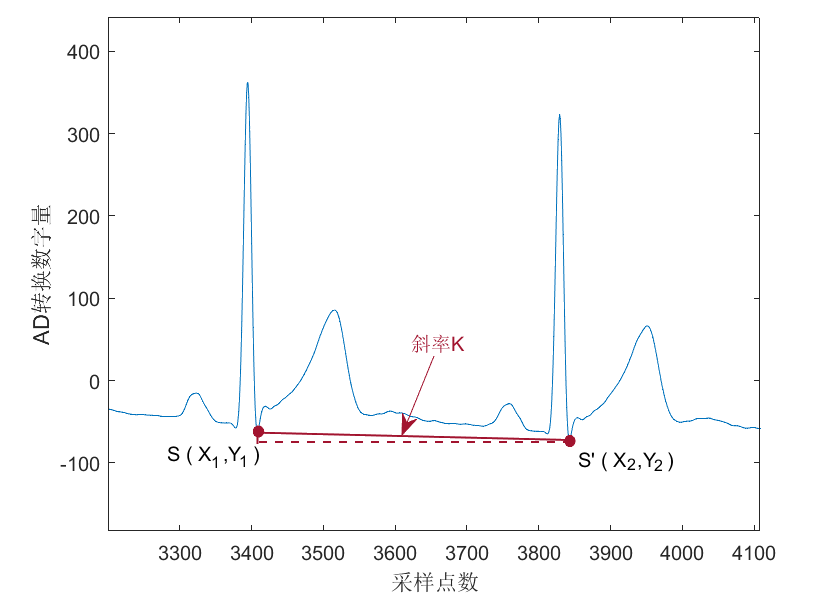
\includegraphics[width=.74\linewidth]{baseline_drift_removing.png}
    \caption[去除基线漂移示意图]{去除基线漂移示意图}
    \label{fig:Baseline-drift-removing}
\end{figure}

(4)标准化

为提高被试间数据的可比性,最后采用Z-Score标准化消除被试间差异,计算公式为:
\vspace{-2ex}
\begin{equation}
    \label{equ:Mean}
    \tilde{X}=\frac{X-\mu}{\sigma}
    % \vspace{-1ex}
\end{equation}

其中μ和σ分别为信号的均值和标准差,标准化后的信号\~X,符合标准正态分布(即均值为0、标准差为1)。

以下选取一段预处理后的心电信号和对应原始信号进行展示(如\autoref{fig:ECG-pretreat}所示),时间轴未对齐是因为预处理中将心电信号第一个波谷前的小段信号删去了。
\vspace{-1ex}
\begin{figure}[htbp]
    \makebox[\textwidth][c]{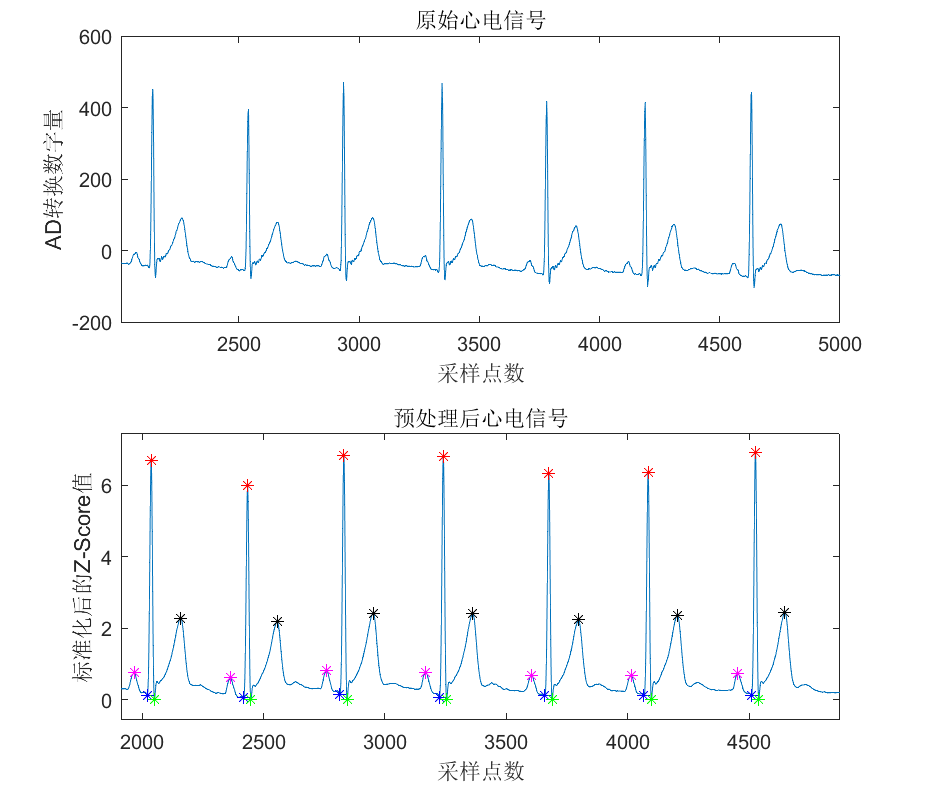
\includegraphics[width=0.82\textwidth]{ECG-pretreat.png}}
    \caption[心电信号预处理示意图]{心电信号预处理示意图}
    \label{fig:ECG-pretreat}
\end{figure}

\subsubsection{脉搏波信号预处理}
脉搏波信号的预处理流程与心电信号类似,使用五点三次平均法进行平滑处理后,定位波峰波谷,并在相邻波谷间采用与心电信号相同的数学方法去除基线漂移,
最后使用Z-Score方法进行标准化处理。波峰波谷的提取过程为:首先通过原始脉搏波信号的一阶差分值在移动窗(宽度设为24)内寻找局部峰值点,
返回的所有峰值点除脉搏波波峰外,还包括大量重搏波波峰。对所有局部峰值点进行以下判断以剔除重搏波波峰的特征点:

1. 计算每个局部峰值点与波谷的幅值之差,去除幅值之差小于所设阈值的点(阈值设为0.55倍前一个波峰波谷幅值之差);

2. 计算相邻两局部峰值点之间的距离,去除距离小于所设阈值的后一个局部峰值点(阈值设为0.3倍采样率,即脉率上限设置为200);

3. 计算每个局部峰值点与前后两波谷幅值之差的比值,若比值不在设定范围内,删除该局部峰值点所在脉搏波的所有特征点(理想状态下相邻两波谷位于同一水平线,即比值为1,本研究中范围设定为0.5$ \sim $2)。

通过以上步骤,重搏波波峰被全部去除。波峰定位完成后,相邻两波峰之间的极小值点即为波谷。
% 预处理后的脉搏波信号如\autoref{fig:PPG-pretreat}所示。
以下选取一段预处理后的脉搏波信号和对应原始信号进行展示(如\autoref{fig:PPG-pretreat}所示),时间轴未对齐是因为预处理中将脉搏波信号第一个波谷前的小段信号删去了。
\vspace{-1ex}
% \begin{table}[!htb]
\begin{figure}[htbp]
    \makebox[\textwidth][c]{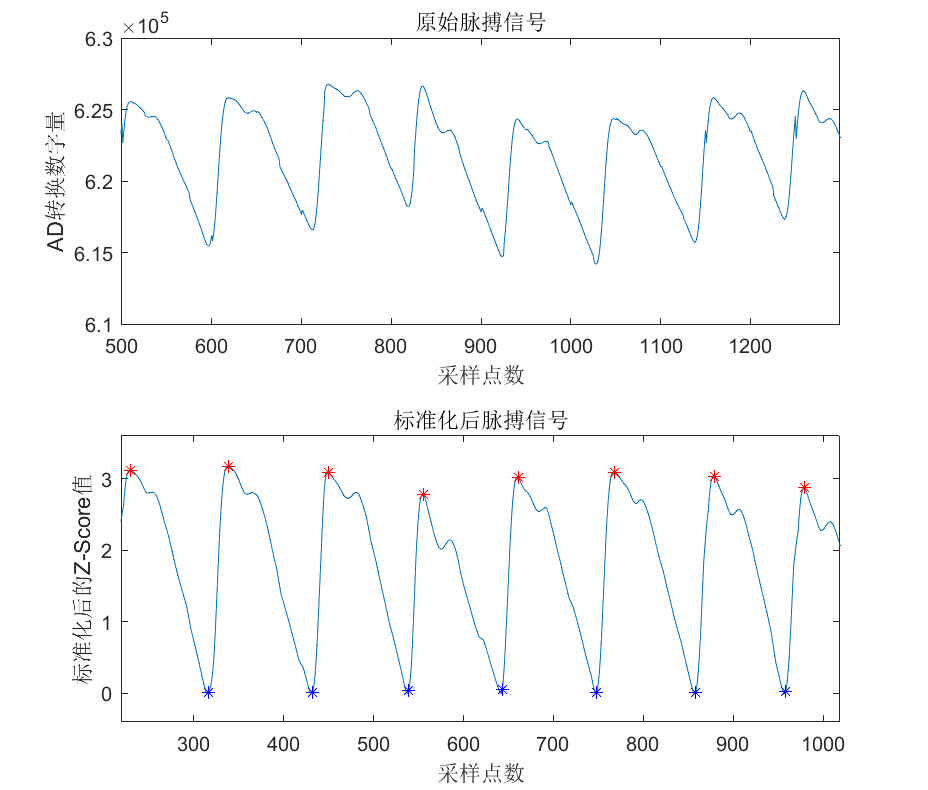
\includegraphics[width=0.82\textwidth]{PPG-pretreat.png}}
    \caption[脉搏波信号预处理示意图]{脉搏波信号预处理示意图}
    \label{fig:PPG-pretreat}
\end{figure}
% \end{table}

\subsubsection{呼吸信号预处理}
呼吸信号的预处理流程同样与心电信号类似,使用五点三次平均法和50Hz带陷滤波器处理后,通过设置findpeaks函数的最小间隔限制
(相邻局部峰值点间距离不小于1.6倍采样率)定位波峰波谷,最后使用Z-Score方法对信号进行标准化处理。
% 预处理后的呼吸信号如\autoref{fig:RESP-pretreat}所示。
以下选取一段预处理后的呼吸信号和对应原始信号进行展示(如\autoref{fig:RESP-pretreat}所示),时间轴未对齐是因为预处理中将呼吸信号第一个波谷前的小段信号删去了。

\begin{figure}[htbp]
    \makebox[\textwidth][c]{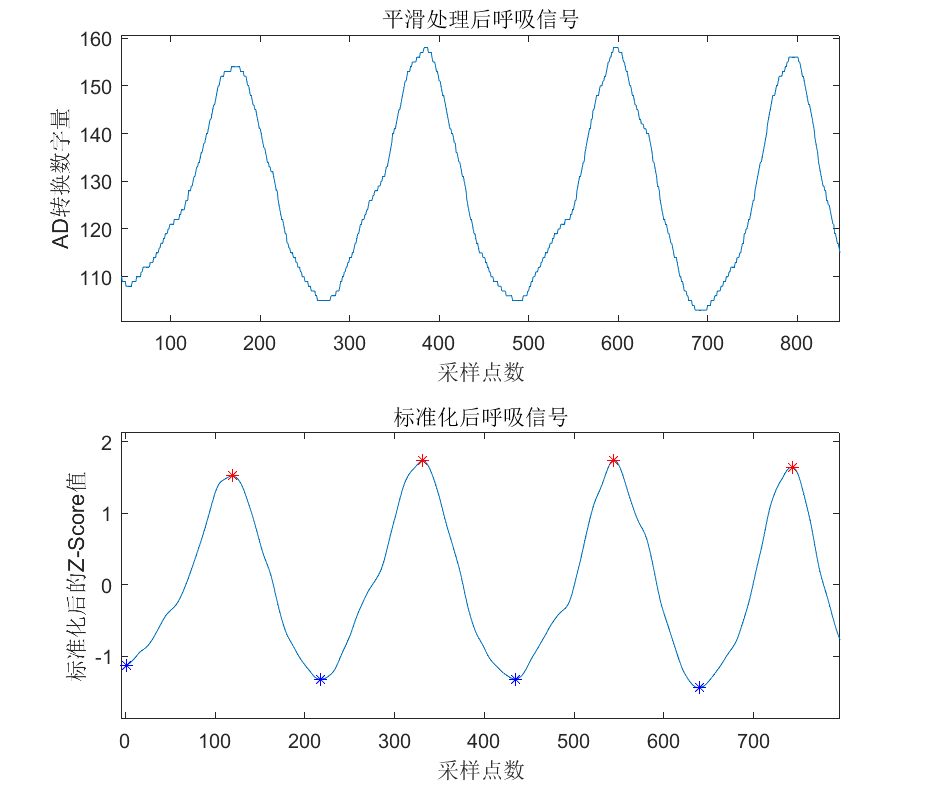
\includegraphics[width=0.82\textwidth]{RESP-pretreat.png}}
    \caption[呼吸信号预处理示意图]{呼吸信号预处理示意图}
    \label{fig:RESP-pretreat}
\end{figure}

\subsection{特征提取}
情绪状态改变时,外周生理信号的形态特征、能量分布以及复杂和混乱程度等都可能发生相应的变化。参考近年来国内外研究中的常用特征,
本研究从标准化后的心电、脉搏波和呼吸信号中提取了时域、频域和非线性三个维度共80个情绪特征。

\subsubsection{时域特征}
探究外周生理信号在不同情绪状态下的改变时,波形的形态特征最为直观,例如情绪紧张导致心率、脉率和呼吸频率改变时,相应信号的波形宽度及幅度均会发生相应的改变。
本研究提取的时域特征包括信号均值、标准差、一/二阶差分、变异系数和统计学特征等九类时域特征,计算公式如下:

(1)信号均值
\begin{equation}
    \label{equ:Mean}
    \mu_{X}=\frac{1}{N} \sum_{n=1}^{N} X_{n}
    % \vspace{-1ex}
\end{equation}

(2)信号标准差
\begin{equation}
    \label{equ:STD}
    \sigma_{X}=\left(\frac{1}{N-1} \sum_{n=1}^{N}\left(X_{n}-\mu_{X}\right)^{2}\right)^{\frac{1}{2}}
    % \vspace{-1ex}
\end{equation}

(3)信号一阶差分绝对值的均值
\vspace{-1ex}
\begin{equation}
    \label{equ:Delta}
    \delta_{X}=\frac{1}{N-1} \sum_{n=1}^{N-1}\left|X_{n+1}-X_{n}\right|=\frac{\delta_{X}}{\sigma_{X}}
    \vspace{-1ex}
\end{equation}

(4)信号二阶差分绝对值的均值
\vspace{-1ex}
\begin{equation}
    \label{equ:Gamma}
    \gamma_{X}=\frac{1}{N-2} \sum_{n=1}^{N-2}\left|X_{n+2}-X_{n}\right|=\frac{\gamma_{X}}{\sigma_{X}}
    \vspace{-1ex}
\end{equation}

(5)变异系数
\begin{equation}
    \label{equ:Sigma}
    \text { CV }=\frac{\sigma_{X}}{\mu_{X}} * 100 \%
    % \vspace{-1ex}
\end{equation}

(6)峰度系数(Kurtosis,表征数据分布的尖峰和扁平程度)
\vspace{-1ex}
\begin{equation}
    \label{equ:Kurtosis}
    \text { Kurtosis }=\frac{\frac{1}{N} \sum_{n=1}^{N}\left(X_{n}-\mu_{X}\right)^{4}}{\left(\frac{1}{N} \sum_{n=1}^{N}\left(X_{n}-\mu_{X}\right)^{2}\right)^{2}}-3
    \vspace{-1ex}
\end{equation}

(7)偏度系数(Skewness,表征数据分布的对称性)
\vspace{-1ex}
\begin{equation}
    \label{equ:Skewness}
    \text { Skewness }=\frac{\frac{1}{N} \sum\left(X-\mu_{X}\right)^{3}}{\sigma_{X}^{3}}
    \vspace{-1ex}
\end{equation}

以上特征中,N为样本点数,$X_n$为第n个样本点的值,$X_{n+1}$为第n+1个样本点的值,以此类推。

(8)K值(表征脉搏波波形和面积变化)\cite{罗志昌1996脉搏波波形特征信息的研究}
\vspace{-1ex}
\begin{equation}
    \label{equ:K-value}
    K=\displaystyle{\frac{P_{m}-P_{\mathrm{d}}}{P_{\mathrm{s}}-P_{\mathrm{d}}}}
    \vspace{-4ex}
\end{equation}
\begin{equation}
    \label{equ:K-value}
    P_{m}=\frac{1}{T} \int_{0}^{T} P(t) d t
\end{equation}

其中$P_m$为平均动脉压(一个脉搏波周期内脉搏压力的均值),$P_s$和$P_d$分别为脉搏波波峰值(收缩压)和波谷值(舒张压)。类比心电信号,则对应计算R波和S波以及信号均值之间的关系,以反映心电信号QRS波群的能量占比\cite{陈沙利2021}。

(9)光电容积斜率指数(PSI)\cite{陈婉琳2019脉搏波形态学研究及其在子痫前期的应用}

将脉搏波波形的下降支横坐标十等分,即$P_0$ ($X_0$, $Y_0$) $\sim $ $P_{10}$ ($X_{10}$, $Y_{10}$)。光电容积斜率指数${PSI}_{ij}$表示$P_i$($X_i$, $Y_i$)和$P_j$($X_j$, $Y_j$)两点间连线斜率,计算公式如下:
\vspace{-1ex}
\begin{equation}
    \label{equ:K-value}
    \left\{\begin{array}{c}
        k=\displaystyle{\frac{Y_{0}-Y_{10}}{X_{0}-X_{10}}} \\
        \vspace{-2ex}
        \\
        {P S I}_{i j}=\displaystyle{\frac{k_{i j}}{k}}=\displaystyle{\frac{Y_{j}-Y_{i}}{\left(X_{j}-X_{i}\right) k}}
    \end{array}\right.
\end{equation}

\subsubsection{频域特征}
虽然幅值、频率等时域信息可以直观表现信号的形态特征,但生理信号还具有非常重要的非平稳特性,因此各研究还在时域特征的基础上探索生理信号在频域上的表现,以获得更多更全面的信号特征。
例如,心电信号的低频和高频谱段功率及两者比值分别可以反映交感神经系统、副交感神经系统以及两者的均衡性或平衡性。
本研究运用Burg法进行功率谱密度估计并在此基础上计算各频率段内的信号功率作为主要的频域特征。

功率谱密度(PSD)描述了信号功率在频域中的分布情况,计算公式为:
\vspace{-1ex}
\begin{equation}
    \label{equ:K-value}
        P_{x x}(w)=\frac{1}{2 \pi} \sum_{m=-\infty}^{+\infty} R_{x x}(m) e^{-j w m}
        \vspace{-1ex}
\end{equation}

其中$R_{xx}$(m)为信号自相关序列,即PSD是$R_{xx}$(m)进行离散时间傅里叶变换所得。
通过对PSD在某频率范围[ $\omega_1$, $\omega_2$ ] ( 0 ≤ $\omega_1$ ≤ $\omega_2 $≤ $\pi$ )内的积分,可以进一步求得信号在该频率范围内的功率,即:
\begin{equation}
    \label{equ:K-value}
        P_{\left[w_{1}, w_{2}\right]}=\int_{w_{1}}^{w_{2}} R_{x x}(w) d w
\end{equation}

目前,功率谱估计方法主要分为经典谱估计方法(非参数化方法,包括周期图法、自相关法、平均法、Welch法等)和现代谱估计方法
(参数化方法,包括自回归模型法、多重信号分类法、Burg法等),后者较前者在频率分辨率和方差上均有很大的改善。
现代谱估计中的Burg法是利用线性预测与AR(M)模型互为逆系统的原理推导所得\cite{刘金星2016现代谱估计技术的研究应用与},能够利用有限数据直接估计前后向线性预测参数,
且无需计算自相关函数,估计精度高而计算量小,在研究中被广泛使用,本研究也选用该方法进行功率谱估计。

\subsubsection{非线性特征}
除常规的时域和频域特征外,生理信号还具有非常复杂的非线性特征,这些特征与大脑、神经和心脏等部位的活动高度相关,
可以反映情绪的调控过程\cite{陈沙利2021}。相关研究证明\cite{2012The},单独使用非线性特征或将其与传统时频域特征融合均能有效构建或优化情绪分类模型。
本研究提取了信息熵(近似熵、样本熵、小波熵、谱熵)、关联维数和Lempel-Ziv复杂度三种非线性特征。

(1)信息熵

信息熵表征随机变量的不确定性或信息量大小,具有单调性(事件发生概率越高,其携带信息量越低)、非负性和累加性三个特性\cite{Shannon2001A},定义如下:
\vspace{-1ex}
\begin{equation}
    \label{equ:K-value}
    H(X)=-\sum_{i=1}^{n} p\left(x_{i}\right) \log p\left(x_{i}\right)
    \vspace{-1ex}
\end{equation}

其中$x_i$为事件的n种可能情况且每种情况彼此独立,$p_i$为$x_i$情况对应出现的概率。
如果事件可能出现的情况种类很少(如只出现1种情况,则对应概率为1,信息熵为0),则信息熵较小,表示事件的不确定性和复杂度较低。

信息熵的表现形式很多,论文采用MATLAB EntropyHub工具包分别计算得到近似熵、样本熵、小波熵和谱熵四类熵值。其中,
近似熵(ApEn)反映时间序列的复杂性和产生新信息的可能性;
样本熵(SampEn)与近似熵的物理意义相似,通过度量信号中产生新模式的概率大小来衡量时间序列的复杂性,即产生新模式的概率越大,序列的复杂性就越大\cite{杨晓利2014肌电信号的样本熵分析};
小波熵(WeEn)反映信号在不同尺度上的能量分布;
谱熵(SeEn)反映信号能量在频域上的不确定性,即信号能量分布越均匀,信号的不确定性和复杂度越大。

(2)关联维数

关联维数表征系统中相点之间的相关度和自相似性,是非线性动力学系统中的一种典型特征。
论文采用Grassberger和Procaccia在1983年提出的G-P算法\cite{1983Characterization}计算关联维数,具体过程如下。

首先定义关联积分函数C(r)为:
\vspace{-2ex}
\begin{equation}
    \label{equ:K-value}
    C(r)=\frac{1}{N(N-1)} \sum_{i=1, i \neq j}^{N} \sum_{j=1}^{N} H\left(r-\left\|X_{i}-X_{j}\right\|\right)
    \vspace{-1ex}
\end{equation}

其中H为Heaviside阶跃函数,${\left\|X_{i}-X_{j}\right\|}$为两点间距离。则关联维数D为:
\vspace{-1ex}
\begin{equation}
    \label{equ:K-value}
    D=\lim _{r \rightarrow 0} \frac{\ln C(r)}{\ln r}
    \vspace{-1ex}
\end{equation}

(3)Lempel-Ziv复杂度

Lempel-Ziv复杂度表征时间序列中出现新模式的速度\cite{陈东伟2014情感识别中脑电信号},使用数据量少且抗干扰性强,对于分析非平稳的生理信号很有帮助。
计算时,首先需要对数据进行二值化处理,将信号转化为有限的0-1序列,再计算Lempel-Ziv复杂度,公式定义如下:
\vspace{-1ex}
\begin{equation}
    \label{equ:K-value}
    L Z=C(S) \frac{\log _{2}(S)}{S}
    \vspace{-1ex}
\end{equation}

其中C(S)表示长度为S的0-1序列中出现新模式的个数。

\subsubsection{原始特征集}
本研究从心电、脉搏波和呼吸信号中共提取到时域、频域和非线性三个维度的80个特征,以探究不同情绪状态与外周生理信号的形态特征、能量分布以及复杂和混乱程度等特征之间的关联。
需要注意的是,所有特征均在原有基础上减去了相应的基线值(每位被试所有平静状态下的特征对应取平均值记为该被试该特征的基线值),即取所有特征相对基线的变化量构成最终的原始特征集。
提取的所有特征及其含义分别汇总如\autoref{tab:ECG-Feature-Summary}、\autoref{tab:PPG-Feature-Summary}和\autoref{tab:RESP-Feature-Summary}。


% \tablecaption{心电信号提取特征汇总表}
% \tablehead
% {\hline \\ \bfseries 维度&\bfseries 特征名称&\bfseries 特征含义\\ \hline}
% \tabletail
% {\hline}
% \tablelasttail{\bottomrule}
% \begin{supertabular}{lll}
%     \multirow{10}{*}{\textbf{\begin{tabular}[c]{@{}l@{}}时域特征\\ (10个)\end{tabular}}} & {ECG\_NN\_mean}         & {RR间期序列均值}                     \\
%                                                           & {ECG\_SDNN}             & {RR间期序列标准差}                   \\
%                                                           & {ECG\_rMSSD}            & {相邻RR间期差值的均方}               \\
%                                                           & {ECG\_RR\_CV}           & {RR间期序列变异性}                   \\
%                                                           & {ECG\_pNN50}            & {\begin{tabular}[c]{@{}l@{}}相邻RR间期差值大于50ms的个数\\ 占总RR间期的百分比\end{tabular}}         \\
%                                                           & {ECG\_K}                & {心电信号K值}                        \\
%                                                           & {HR\_Delta}             & {心率序列一阶差分绝对值均值}         \\
%                                                           & {HR\_Gamma}             & {心率序列二阶差分绝对值均值}         \\
%                                                           & {HR\_kurto}             & {心率序列峰度系数}                   \\
%                                                           & {HR\_skewness}          & {心率序列偏度系数}                   \\ \midrule
%     \multirow{6}{*}{\textbf{\begin{tabular}[c]{@{}l@{}}频域特征\\ (6个)\end{tabular}}}  & {ECG\_VLF}              & {极低频段能量(0$ \sim $0.04Hz)}    \\
%                                                           & {ECG\_LF}               & {低频段能量(0.04$ \sim $0.15Hz)}   \\
%                                                           & {ECG\_HF}               & {高频段能量(0.15$ \sim $0.4Hz)}    \\
%                                                           & {ECG\_LF\_norm}         & {低频段能量标准化(LF/(LF+HF)*100)} \\
%                                                           & {ECG\_HF\_norm}         & {高频段能量标准化(HF/(LF+HF)*100)} \\
%                                                           & {ECG\_Power\_ratio}     & {低高频段能量之比}                   \\ \midrule
%     \multirow{10}{*}{\textbf{\begin{tabular}[c]{@{}l@{}}非线性特征\\ (10个)\end{tabular}}} & {ECG\_ApEn}           & {近似熵}                             \\
%                                                           & {ECG\_SampEn}             & {样本熵}                             \\
%                                                           & {ECG\_WeEn\_shannon}    & {小波熵-香农熵}                      \\
%                                                           & {ECG\_WeEn\_log}        & {小波熵-对数能量熵}                  \\
%                                                           & {ECG\_WeEn\_threshold}  & {小波熵-阈值熵}                      \\
%                                                           & {ECG\_WeEn\_sure}       & {小波熵-范数熵}                      \\
%                                                           & {ECG\_WeEn\_norm}       & {小波熵-范数熵}                      \\
%                                                           & {ECG\_SeEn}             & {谱熵}                               \\
%                                                           & {ECG\_corDim}           & {关联维数}                           \\
%                                                           & {ECG\_RR\_LZComplexity} & {RR间期序列Lempel-Ziv复杂度}         \\ 
% \end{supertabular}{lll}
\clearpage
\makeatletter
\setlength{\@fptop}{5pt}
\makeatother
\begin{table}[t]
    \centering
    \footnotesize
    \setlength{\abovecaptionskip}{0.1cm}
    \setlength{\belowcaptionskip}{0.2cm}
    \renewcommand\arraystretch{1.5}
    \caption[心电信号提取特征汇总表]{心电信号提取特征汇总表}
    \label{tab:ECG-Feature-Summary}
    \setlength{\tabcolsep}{0.8cm}{
        \begin{tabular}{lll}
            \toprule
            \textbf{维度}                                         & \textbf{特征名称}       & \textbf{特征含义}                    \\ \midrule
            \multirow{10}{*}{\textbf{\begin{tabular}[c]{@{}l@{}}时域特征\\ (10个)\end{tabular}}} & {ECG\_NN\_mean}         & {RR间期序列均值}                     \\
                                                                  & {ECG\_SDNN}             & {RR间期序列标准差}                   \\
                                                                  & {ECG\_rMSSD}            & {相邻RR间期差值的均方}               \\
                                                                  & {ECG\_RR\_CV}           & {RR间期序列变异性}                   \\
                                                                  & {ECG\_pNN50}            & {\begin{tabular}[c]{@{}l@{}}相邻RR间期差值大于50ms的个数\\ 占总RR间期的百分比\end{tabular}}         \\
                                                                  & {ECG\_K}                & {心电信号K值}                        \\
                                                                  & {HR\_Delta}             & {心率序列一阶差分绝对值均值}         \\
                                                                  & {HR\_Gamma}             & {心率序列二阶差分绝对值均值}         \\
                                                                  & {HR\_kurto}             & {心率序列峰度系数}                   \\
                                                                  & {HR\_skewness}          & {心率序列偏度系数}                   \\ \midrule
            \multirow{6}{*}{\textbf{\begin{tabular}[c]{@{}l@{}}频域特征\\ (6个)\end{tabular}}}  & {ECG\_VLF}              & {极低频段能量(0$ \sim $0.04Hz)}    \\
                                                                  & {ECG\_LF}               & {低频段能量(0.04$ \sim $0.15Hz)}   \\
                                                                  & {ECG\_HF}               & {高频段能量(0.15$ \sim $0.4Hz)}    \\
                                                                  & {ECG\_LF\_norm}         & {低频段能量标准化(LF/(LF+HF)*100)} \\
                                                                  & {ECG\_HF\_norm}         & {高频段能量标准化(HF/(LF+HF)*100)} \\
                                                                  & {ECG\_Power\_ratio}     & {低高频段能量之比}                   \\ \midrule
            \multirow{10}{*}{\textbf{\begin{tabular}[c]{@{}l@{}}非线性特征\\ (10个)\end{tabular}}} & {ECG\_ApEn}           & {近似熵}                             \\
                                                                  & {ECG\_SampEn}             & {样本熵}                             \\
                                                                  & {ECG\_WeEn\_shannon}    & {小波熵-香农熵}                      \\
                                                                  & {ECG\_WeEn\_log}        & {小波熵-对数能量熵}                  \\
                                                                  & {ECG\_WeEn\_threshold}  & {小波熵-阈值熵}                      \\
                                                                  & {ECG\_WeEn\_sure}       & {小波熵-范数熵}                      \\
                                                                  & {ECG\_WeEn\_norm}       & {小波熵-范数熵}                      \\
                                                                  & {ECG\_SeEn}             & {谱熵}                               \\
                                                                  & {ECG\_corDim}           & {关联维数}                           \\
                                                                  & {ECG\_RR\_LZComplexity} & {RR间期序列Lempel-Ziv复杂度}         \\ \bottomrule
        \end{tabular}}
\end{table}
\clearpage
\makeatletter
\setlength{\@fptop}{5pt}
\makeatother
\begin{table}[t]
    \centering
    \footnotesize
    \setlength{\abovecaptionskip}{0.1cm}
    \setlength{\belowcaptionskip}{0.2cm}
    \renewcommand\arraystretch{1.5}
    \caption[脉搏波信号提取特征汇总表]{脉搏波信号提取特征汇总表}
    \label{tab:PPG-Feature-Summary}
    \setlength{\tabcolsep}{0.8cm}{
        \begin{tabular}{lll}
            \toprule
            \textbf{维度}                                         & \textbf{特征名称}       & \textbf{特征含义}                        \\ \midrule
            \multirow{14}{*}{\textbf{\begin{tabular}[c]{@{}l@{}}时域特征\\ (14个)\end{tabular}}} & {PPG\_mean}             & {脉搏波信号均值}                         \\
                                                                  & {PPG\_PP\_mean}         & {PP间期(相邻脉搏波波峰时间差)序列均值} \\
                                                                  & {PPG\_PP\_std}          & {PP间期序列标准差}                       \\
                                                                  & {PPG\_Delta}            & {脉搏波信号一阶差分绝对值均值}           \\
                                                                  & {PPG\_Gamma}            & {脉搏波信号二阶差分绝对值均值}           \\
                                                                  & {PPG\_PP\_Delta}        & {PP间期序列一阶差分绝对值均值}           \\
                                                                  & {PPG\_PP\_Gamma}        & {PP间期序列二阶差分绝对值均值}           \\
                                                                  & {PPG\_PP\_CV}           & {PP间期序列变异性}                       \\
                                                                  & {PPG\_K}                & {脉搏波信号K值}                          \\
                                                                  & {PPG\_PP\_Kurto}        & {PP间期序列峰度系数}                     \\
                                                                  & {PPG\_PP\_Skewness}     & {PP间期序列偏度系数}                     \\
                                                                  & {PPG\_PSI38}            & {光电容积斜率指数}                       \\
                                                                  & {PPG\_PSI39}            & {光电容积斜率指数}                       \\
                                                                  & {PPG\_PSI310}           & {光电容积斜率指数}                       \\ \midrule
            \multirow{6}{*}{\textbf{\begin{tabular}[c]{@{}l@{}}频域特征\\ (6个)\end{tabular}}}  & {PPG\_VLF}              & {极低频段能量(0$ \sim $0.04Hz)}        \\
                                                                  & {PPG\_LF}               & {低频段能量(0.04$ \sim $0.15Hz)}       \\
                                                                  & {PPG\_HF}               & {高频段能量(0.15$ \sim $0.4Hz)}        \\
                                                                  & {PPG\_LF\_norm}         & {低频段能量标准化(LF/(LF+HF)*100)}     \\
                                                                  & {PPG\_HF\_norm}         & {高频段能量标准化(HF/(LF+HF)*100)}     \\
                                                                  & {PPG\_Power\_ratio}     & {低高频段能量之比}                       \\ \midrule
            \multirow{10}{*}{\textbf{\begin{tabular}[c]{@{}l@{}}非线性特征\\ (10个)\end{tabular}}} & {PPG\_ApEn}           & {近似熵}                                 \\
                                                                  & {PPG\_SampEn}             & {样本熵}                                 \\
                                                                  & {PPG\_WeEn\_shannon}    & {小波熵-香农熵}                          \\
                                                                  & {PPG\_WeEn\_log}        & {小波熵-对数能量熵}                      \\
                                                                  & {PPG\_WeEn\_threshold}  & {小波熵-阈值熵}                          \\
                                                                  & {PPG\_WeEn\_sure}       & {小波熵-范数熵}                          \\
                                                                  & {PPG\_WeEn\_norm}       & {小波熵-范数熵}                          \\
                                                                  & {PPG\_SeEn}             & {谱熵}                                   \\
                                                                  & {PPG\_corDim}           & {关联维数}                               \\
                                                                  & {PPG\_PP\_LZComplexity} & {PP间期序列Lempel-Ziv复杂度}             \\ \bottomrule
        \end{tabular}}
\end{table}
\clearpage
\makeatletter
\setlength{\@fptop}{5pt}
\makeatother
\begin{table}[t]
    \centering
    \footnotesize
    \setlength{\abovecaptionskip}{0.1cm}
    \setlength{\belowcaptionskip}{0.2cm}
    \renewcommand\arraystretch{1.5}
    \caption[呼吸信号提取特征汇总表]{呼吸信号提取特征汇总表}
    \label{tab:RESP-Feature-Summary}
    \setlength{\tabcolsep}{0.8cm}{
        \begin{tabular}{lll}
            \toprule
            \textbf{维度}                                         & \textbf{特征名称}        & \textbf{特征含义}                          \\ \midrule
            \multirow{9}{*}{\textbf{\begin{tabular}[c]{@{}l@{}}时域特征\\ (9个)\end{tabular}}}  & {RESP\_mean}             & {呼吸信号均值}                             \\
                                                                  & {RESP\_PP\_mean}         & {PP间期(相邻呼吸信号波峰时间差)序列均值} \\
                                                                  & {RESP\_AMP\_mean}        & {呼吸幅值序列均值}                         \\
                                                                  & {RESP\_PP\_std}          & {PP间期序列标准差}                         \\
                                                                  & {RESP\_AMP\_std}         & {呼吸幅值序列标准差}                       \\
                                                                  & {RESP\_Delta}            & {呼吸信号一阶差分绝对值均值}               \\
                                                                  & {RESP\_Gamma}            & {呼吸信号二阶差分绝对值均值}               \\
                                                                  & {RESP\_RV\_amp}          & {呼吸幅值变异性}                           \\
                                                                  & {RESP\_RV\_fre}          & {呼吸频率变异性}                           \\ \midrule
            \multirow{5}{*}{\textbf{\begin{tabular}[c]{@{}l@{}}频域特征\\ (5个)\end{tabular}}}  & {RESP\_LF}               & {低频段能量(0.05$ \sim $0.25Hz)}         \\
                                                                  & {RESP\_HF}               & {高频段能量(0.25$ \sim $5Hz)}            \\
                                                                  & {RESP\_LF\_norm}         & {低频段能量标准化(LF/(LF+HF)*100)}       \\
                                                                  & {RESP\_HF\_norm}         & {高频段能量标准化(HF/(LF+HF)*100)}       \\
                                                                  & {RESP\_Power\_ratio}     & {低高频段能量之比}                         \\ \midrule
            \multirow{10}{*}{\textbf{\begin{tabular}[c]{@{}l@{}}非线性特征\\ (10个)\end{tabular}}} & {RESP\_ApEn}           & {近似熵}                                   \\
                                                                  & {RESP\_SampEn}             & {样本熵}                                   \\
                                                                  & {RESP\_WeEn\_shannon}    & {小波熵-香农熵}                            \\
                                                                  & {RESP\_WeEn\_log}        & {小波熵-对数能量熵}                        \\
                                                                  & {RESP\_WeEn\_threshold}  & {小波熵-阈值熵}                            \\
                                                                  & {RESP\_WeEn\_sure}       & {小波熵-范数熵}                            \\
                                                                  & {RESP\_WeEn\_norm}       & {小波熵-范数熵}                            \\
                                                                  & {RESP\_SeEn}             & {谱熵}                                     \\
                                                                  & {RESP\_corDim}           & {关联维数}                                 \\
                                                                  & {RESP\_PP\_LZComplexity} & {PP间期序列Lempel-Ziv复杂度}               \\ \bottomrule
        \end{tabular}}
\end{table}

至此,本研究构建完成了包含心电、脉搏波和呼吸三种外周生理信号以及时域、频域和非线性三个维度共80个特征的原始特征集,以进行后续的统计学分析和分类模型构建。

\clearpage
\section{有效特征的统计学分析}

为探究原始特征集在不同情绪状态下的表征是否具有显著性差异,本研究对所有提取的生理特征进行了统计学分析。

\subsection{统计显著性}

\begin{spacing}{1.5} 
由于原始特征集的总体样本量较小且分布类型未知,无法确定特征集的类间总体方差是否相等以及是否来自于正态分布总体,
因此本研究采用非参数检验中的曼-惠特尼U检验(Menn-Whitney U test)对三种情绪状态及其特征集进行独立样本分析。
U检验假设两个样本分别来自除了总体均值以外完全相同的两个总体,目的是检验这两个总体的均值是否有显著的差别,主要用于不满足正态分布的小样本。

原始特征集的统计检验结果如\autoref{tab:P-value}所示(满足显著性标准的特征在表内优先展示),P值加粗表示该特征在对应二分类任务的组间分布具有显著性差异,其中*表示p<0.05,**表示p<0.01,***表示p<0.001。
\end{spacing}
\vspace{-1ex}
% Please add the following required packages to your document preamble:
% \usepackage[table,xcdraw]{xcolor}
% If you use beamer only pass "xcolor=table" option, i.e. \documentclass[xcolor=table]{beamer}
% {\small 
\begin{footnotesize}
\begin{longtable}[htbp]{m{4.5cm}<{\raggedright}m{3cm}<{\raggedright}m{3cm}<{\raggedright}m{2.2cm}<{\raggedright}}
    % \centering  \\
    % \footnotesize  \\
    % \fontsize{10}{4}                                                                                          \\
    % \renewcommand\arraystretch{1.5}  \\
    \caption[原始特征集在各分类任务中的非参数检验结果]{原始特征集在各分类任务中的非参数检验结果(α=0.05)}  
    \vspace{-2ex}                                   \\
    \label{tab:P-value}                                                                                                                \\
    \toprule
    \textbf{特征}                      & \textbf{P(恐惧平静)}          & \textbf{P(愉悦平静)}          & \textbf{P(恐惧愉悦)}          \\
    \hline
    \endfirsthead
    \caption[]{(续)}                                                                                                                   \\
    % \hline
    \toprule
    \textbf{特征}                      & \textbf{P(恐惧平静)}          & \textbf{P(愉悦平静)}          & \textbf{P(恐惧愉悦)}          \\
    \hline
    \endhead
    \hline
    \endfoot
    \bottomrule
    \endlastfoot
    % \begin{tabular}{llll}
    % \toprule
    % \makebox[0.3\textwidth][l]{特征} & \makebox[0.2\textwidth][l]{恐惧平静}
    %                                  & \makebox[0.2\textwidth][l]{愉悦平静} & \makebox[0.1\textwidth][l]{恐惧愉悦} \\
    %{ \textbf{特征}}                   & \multicolumn{1}{l}{{ \textbf{P(恐惧平静)}}} & \multicolumn{1}{l}{{ \textbf{P(愉悦平静)}}} & \multicolumn{1}{l}{{ \textbf{P(恐惧愉悦)}}} \\
    % \midrule
    { \textbf{ECG\_corDim}}            & { \boldmath{$0.0360^{*}$}}    & {  \boldmath{$0.0000^{***}$}} & {  \boldmath{$0.0190^{*}$}}   \\
    { \textbf{ECG\_RR\_LZComplexity}}  & { \boldmath{$0.0250^{*}$}}    & {  \boldmath{$0.0000^{***}$}} & {  \boldmath{$0.0000^{***}$}} \\
    { \textbf{PPG\_K}}                 & {  \boldmath{$0.0000^{***}$}} & {  \boldmath{$0.0000^{***}$}} & { 0.4750}                     \\
    { \textbf{PPG\_PP\_Kurto}}         & {  \boldmath{$0.0500^{*}$}}   & {  \boldmath{$0.0398^{*}$}}   & { 0.6720}                     \\
    { \textbf{PPG\_VLF}}               & {  \boldmath{$0.0200^{*}$}}   & {  \boldmath{$0.0001^{***}$}} & { 0.7470}                     \\
    { \textbf{PPG\_LF\_norm}}          & {  \boldmath{$0.0000^{***}$}} & {  \boldmath{$0.0000^{***}$}} & { 0.6760}                     \\
    { \textbf{PPG\_HF\_norm}}          & {  \boldmath{$0.0000^{***}$}} & {  \boldmath{$0.0000^{***}$}} & { 0.6760}                     \\
    { \textbf{PPG\_Power\_ratio}}      & {  \boldmath{$0.0000^{***}$}} & {  \boldmath{$0.0000^{***}$}} & { 0.7450}                     \\
    { \textbf{PPG\_SampEn}}            & {  \boldmath{$0.0020^{**}$}}  & {  \boldmath{$0.0002^{***}$}} & { 0.3650}                     \\
    { \textbf{RESP\_Gamma}}            & {  \boldmath{$0.0380^{*}$}}   & {  \boldmath{$0.0002^{***}$}} & { 0.5550}                     \\
    { \textbf{ECG\_NN\_mean}}          & { 0.0750}                     & {  \boldmath{$0.0000^{***}$}} & {  \boldmath{$0.0000^{***}$}} \\
    { \textbf{ECG\_K}}                 & { 0.2460}                     & {  \boldmath{$0.0001^{***}$}} & {  \boldmath{$0.0020^{**}$}}  \\
    { \textbf{ECG\_WeEn\_sure}}        & { 0.1980}                     & {  \boldmath{$0.0191^{*}$}}   & {  \boldmath{$0.0120^{*}$}}   \\
    { \textbf{ECG\_SampEn}}            & { 0.5960}                     & {  \boldmath{$0.0000^{***}$}} & {  \boldmath{$0.0000^{***}$}} \\
    { \textbf{ECG\_ApEn}}              & { 0.8080}                     & {  \boldmath{$0.0000^{***}$}} & {  \boldmath{$0.0000^{***}$}} \\
    { \textbf{RESP\_PP\_std}}          & {  \boldmath{$0.0000^{***}$}} & { 0.5724}                     & {  \boldmath{$0.0000^{***}$}} \\
    { \textbf{RESP\_RV\_fre}}          & {  \boldmath{$0.0000^{***}$}} & { 0.6886}                     & {  \boldmath{$0.0000^{***}$}} \\
    { \textbf{PPG\_Delta}}             & { 0.3990}                     & {  \boldmath{$0.0001^{***}$}} & { 0.1280}                     \\
    { \textbf{PPG\_Gamma}}             & { 0.7610}                     & {  \boldmath{$0.0006^{***}$}} & { 0.1750}                     \\
    { \textbf{PPG\_PP\_mean}}          & { 0.8810}                     & {  \boldmath{$0.0010^{***}$}} & { 0.0680}                     \\
    { \textbf{PPG\_LF}}                & { 0.1250}                     & {  \boldmath{$0.0012^{**}$}}  & { 0.5420}                     \\
    { \textbf{PPG\_SeEn}}              & { 0.6950}                     & {  \boldmath{$0.0242^{*}$}}   & { 0.0700}                     \\
    { \textbf{PPG\_ApEn}}              & { 0.0610}                     & {  \boldmath{$0.0076^{**}$}}  & { 0.7860}                     \\
    { \textbf{PPG\_corDim}}            & { 0.3900}                     & {  \boldmath{$0.0035^{**}$}}  & { 0.2510}                     \\
    { \textbf{PPG\_PP\_LZComplexity}}  & { 0.2910}                     & {  \boldmath{$0.0000^{***}$}} & { 0.1030}                     \\
    { \textbf{ECG\_RR\_CV}}            & {  \boldmath{$0.0330^{***}$}} & { 0.5661}                     & { 0.1780}                     \\
    { \textbf{RESP\_Delta}}            & {  \boldmath{$0.0320^{***}$}} & { 0.0983}                     & { 0.3160}                     \\
    { \textbf{ECG\_WeEn\_threshold}}   & { 0.1270}                     & { 0.0645}                     & {  \boldmath{$0.0250^{*}$}}   \\
    { \textbf{ECG\_WeEn\_norm}}        & { 0.0610}                     & { 0.1366}                     & {  \boldmath{$0.0180^{*}$}}   \\
    { \textbf{RESP\_RV\_amp}}          & { 0.1080}                     & { 0.0916}                     & {  \boldmath{$0.0160^{*}$}}   \\
    { \textbf{ECG\_WeEn\_log}}         & { 0.1440}                     & { 0.0905}                     & {  \boldmath{$0.0380^{*}$}}   \\
    { \textbf{ECG\_SDNN}}              & { 0.0830}                     & { 0.1252}                     & { 0.7110}                     \\
    { \textbf{ECG\_rMSSD}}             & { 0.8490}                     & { 0.7664}                     & { 0.7120}                     \\
    { \textbf{ECG\_pNN50}}             & { 0.0860}                     & { 0.6214}                     & { 0.0530}                     \\
    { \textbf{HR\_Delta}}              & { 0.7770}                     & { 0.2114}                     & { 0.3720}                     \\
    { \textbf{HR\_Gamma}}              & { 0.6090}                     & { 0.5748}                     & { 0.7850}                     \\
    { \textbf{HR\_kurto}}              & { 0.8440}                     & { 0.8126}                     & { 0.6860}                     \\
    { \textbf{HR\_skewness}}           & { 0.6200}                     & { 0.8256}                     & { 0.7110}                     \\
    { \textbf{ECG\_VLF}}               & { 0.5460}                     & { 0.2338}                     & { 0.1990}                     \\
    { \textbf{ECG\_LF}}                & { 0.1260}                     & { 0.6624}                     & { 0.1050}                     \\
    { \textbf{ECG\_HF}}                & { 0.5300}                     & { 0.6325}                     & { 0.4750}                     \\
    { \textbf{ECG\_LF\_norm}}          & { 0.7660}                     & { 0.5788}                     & { 0.5920}                     \\
    { \textbf{ECG\_HF\_norm}}          & { 0.7660}                     & { 0.5788}                     & { 0.5920}                     \\
    { \textbf{ECG\_Power\_ratio}}      & { 0.9620}                     & { 0.5891}                     & { 0.7650}                     \\
    { \textbf{ECG\_WeEn\_shannon}}     & { 0.1900}                     & { 0.1407}                     & { 0.0620}                     \\
    { \textbf{ECG\_SeEn}}              & { 0.3150}                     & { 0.8764}                     & { 0.4090}                     \\
    { \textbf{PPG\_mean}}              & { 0.9190}                     & { 0.3044}                     & { 0.4870}                     \\
    { \textbf{PPG\_PSI38}}             & { 0.5260}                     & { 0.1951}                     & { 0.1350}                     \\
    { \textbf{PPG\_PSI39}}             & { 0.7230}                     & { 0.4096}                     & { 0.2930}                     \\
    { \textbf{PPG\_PSI310}}            & { 0.2430}                     & { 0.1495}                     & { 0.7470}                     \\
    { \textbf{PPG\_PP\_std}}           & { 0.7040}                     & { 0.1062}                     & { 0.1600}                     \\
    { \textbf{PPG\_PP\_CV}}            & { 0.7340}                     & { 0.1259}                     & { 0.2120}                     \\
    { \textbf{PPG\_PP\_Delta}}         & { 0.7220}                     & { 0.0740}                     & { 0.1530}                     \\
    { \textbf{PPG\_PP\_Gamma}}         & { 0.5250}                     & { 0.1356}                     & { 0.1310}                     \\
    { \textbf{PPG\_PP\_Skewness}}      & { 0.2350}                     & { 0.1979}                     & { 0.7470}                     \\
    { \textbf{PPG\_HF}}                & { 0.0510}                     & { 0.9278}                     & { 0.1820}                     \\
    { \textbf{PPG\_WeEn\_shannon}}     & { 0.4250}                     & { 0.6809}                     & { 0.7270}                     \\
    { \textbf{PPG\_WeEn\_log}}         & { 0.7410}                     & { 0.1651}                     & { 0.2880}                     \\
    { \textbf{PPG\_WeEn\_threshold}}   & { 0.8270}                     & { 0.2011}                     & { 0.4980}                     \\
    { \textbf{PPG\_WeEn\_sure}}        & { 0.2610}                     & { 0.5879}                     & { 0.5750}                     \\
    { \textbf{PPG\_WeEn\_norm}}        & { 0.3630}                     & { 0.4584}                     & { 0.8190}                     \\
    { \textbf{RESP\_mean}}             & { 0.6420}                     & { 0.2247}                     & { 0.7630}                     \\
    { \textbf{RESP\_PP\_mean}}         & { 0.2060}                     & { 0.1886}                     & { 0.6980}                     \\
    { \textbf{RESP\_AMP\_mean}}        & { 0.1370}                     & { 0.5053}                     & { 0.2660}                     \\
    { \textbf{RESP\_AMP\_std}}         & { 0.3390}                     & { 0.0975}                     & { 0.0650}                     \\
    { \textbf{RESP\_LF}}               & { 0.2230}                     & { 0.1558}                     & { 0.9050}                     \\
    { \textbf{RESP\_HF}}               & { 0.4360}                     & { 0.8065}                     & { 0.6030}                     \\
    { \textbf{RESP\_LF\_norm}}         & { 0.5820}                     & { 0.5125}                     & { 0.9580}                     \\
    { \textbf{RESP\_HF\_norm}}         & { 0.5820}                     & { 0.5125}                     & { 0.9580}                     \\
    { \textbf{RESP\_Power\_ratio}}     & { 0.4840}                     & { 0.0969}                     & { 0.6980}                     \\
    { \textbf{RESP\_WeEn\_shannon}}    & { 0.2330}                     & { 0.0535}                     & { 0.9520}                     \\
    { \textbf{RESP\_WeEn\_log}}        & { 0.8100}                     & { 0.4016}                     & { 0.5050}                     \\
    { \textbf{RESP\_WeEn\_threshold}}  & { 0.5990}                     & { 0.1270}                     & { 0.1030}                     \\
    { \textbf{RESP\_WeEn\_sure}}       & { 0.4620}                     & { 0.2218}                     & { 0.9560}                     \\
    { \textbf{RESP\_WeEn\_norm}}       & { 0.3230}                     & { 0.4141}                     & { 0.6980}                     \\
    { \textbf{RESP\_SeEn}}             & { 0.4820}                     & { 0.0675}                     & { 0.0570}                     \\
    { \textbf{RESP\_SampEn}}           & { 0.2320}                     & { 0.2610}                     & { 0.6930}                     \\
    { \textbf{RESP\_ApEn}}             & { 0.2380}                     & { 0.1817}                     & { 0.9530}                     \\
    { \textbf{RESP\_corDim}}           & { 0.2840}                     & { 0.4385}                     & { 0.5870}                     \\
    { \textbf{RESP\_PP\_LZComplexity}} & { 0.8930}                     & {\color[HTML]{333333} 0.3148} & {\color[HTML]{333333} 0.6500}
    % \end{tabular}
\end{longtable}
% }
\end{footnotesize}
\vspace{-1ex}
分析上表发现,
经过非参数检验,恐惧平静二分类、愉悦平静二分类和恐惧平静二分类任务分别从原始特征集(80个特征)中筛选出14、26和13个具有显著性差异的特征,
其中愉悦平静二分类任务的有效特征数相对较多且P值更小。
各分类任务的统计学有效特征数总计31个,心电、脉搏波和呼吸信号相关的特征分别为11、15、5个,其中心电和脉搏波相关的有效特征数较多。
三个二分类任务的有效特征汇总如\autoref{tab:Statistic-Feature}所示。
\begin{table}[htbp]
    \centering
    \footnotesize
    \setlength{\abovecaptionskip}{0.1cm}
    \setlength{\belowcaptionskip}{0.2cm}
    \renewcommand\arraystretch{1.5}
    \caption[不同分类任务的统计学有效特征集]{不同分类任务的统计学有效特征集}
    \label{tab:Statistic-Feature}
    \setlength{\tabcolsep}{0.25cm}{
        \begin{tabular}{cl}
            \toprule
            \textbf{分类任务}                                                                     & \textbf{统计学有效特征集}                                                                                                                                                                                                       \\ \midrule
            \multirow{3}{*}[-1.5ex]{\textbf{\begin{tabular}[c]{@{}c@{}}恐惧平静\\ 二分类\\ (14个)\end{tabular}}} & \textbf{\textbf{心电:}}ECG\_RR\_LZComplexity、ECG\_RR\_CV、ECG\_corDim                                                                                                                                                                             \\
                                                                                              & \begin{tabular}[c]{@{}l@{}}\textbf{脉搏波:}PPG\_K、PPG\_PP\_Kurto、PPG\_LF\_norm、PPG\_HF\_norm、PPG\_Power\_ratio、\\ PPG\_VLF、PPG\_SampEn\end{tabular}                                                                                            \\
                                                                                              & \textbf{呼吸:}RESP\_PP\_std、RESP\_RV\_fre、RESP\_Delta、RESP\_Gamma                                                                                                                                                                        \\ \midrule
            \multirow{3}{*}{\textbf{\begin{tabular}[c]{@{}c@{}}\\ 愉悦平静\\ 二分类\\ (26个)\end{tabular}}} & \begin{tabular}[c]{@{}l@{}}\textbf{心电:}ECG\_corDim、ECG\_SampEn、ECG\_ApEn、ECG\_NN\_mean、ECG\_RR\_LZComplexity、\\ ECG\_K、ECG\_WeEn\_sure\end{tabular}                                                                                        \\
                                                                                              & \begin{tabular}[c]{@{}l@{}}\textbf{脉搏波:}PPG\_LF\_norm、PPG\_HF\_norm、PPG\_Power\_ratio、PPG\_K、PPG\_PP\_LZComplexity、\\ PPG\_Delta、PPG\_VLF、PPG\_SampEn、PPG\_Gamma、PPG\_PP\_mean、PPG\_LF、PPG\_corDim、\\ PPG\_ApEn、PPG\_SeEn、PPG\_PP\_Kurto\end{tabular} \\
                                                                                              & \textbf{呼吸:}RESP\_PP\_std、RESP\_RV\_fre、RESP\_RV\_amp、RESP\_Gamma                                                                                                                                                                       \\ \midrule
            \multirow{3}{*}{\textbf{\begin{tabular}[c]{@{}c@{}}恐惧愉悦\\ 二分类\\ (13个)\end{tabular}}} & \begin{tabular}[c]{@{}l@{}}\textbf{心电:}ECG\_NN\_mean、ECG\_SampEn、ECG\_ApEn、ECG\_RR\_LZComplexity、ECG\_K、\\ ECG\_WeEn\_sure、ECG\_WeEn\_norm、ECG\_corDim、ECG\_WeEn\_threshold、ECG\_WeEn\_log\end{tabular}                                             \\
                                                                                              & \textbf{脉搏波:}无                                                                                                                                                                                                                   \\
                                                                                              & \textbf{呼吸:}RESP\_PP\_std、RESP\_RV\_fre、RESP\_RV\_amp         \\ \bottomrule                                                                                                                                                                            
            \end{tabular}}
\end{table}

\subsection{结果分析}
进一步分析分类任务中各特征的非参数检验结果发现:

(1) 从整体上看: 

在具有显著性差异的特征中,心电和脉搏波相关的有效特征占比较大,而呼吸信号相关的占比较小,对情绪分类任务的贡献度可能相对较小。
这表明心电和脉搏波信号与情绪的关联度可能较强而呼吸信号相对较弱。
同时,每种分类任务的统计学有效特征都不完全相同,表明有些特征可能对于多个分类任务有效而另一些特征可能只对单个分类任务有效。

(2) 从单个分类任务来看: 

在恐惧平静二分类任务中,具有显著性差异的特征包括心电信号的1个时域特征、2个非线性特征,脉搏波信号的2个时域特征、4个频域特征、1个非线性特征,
呼吸信号的4个时域特征,脉搏波相关的特征以及时域、频域特征占比较大。

在愉悦平静二分类任务中,具有显著性差异的特征包括心电信号的2个时域特征、5个非线性,脉搏波信号的5个时域特征、5个频域特征、
5个非线性特征,呼吸信号的4个时域,脉搏波相关的特征以及时域、非线性特征占比较大。

在恐惧愉悦二分类任务中,具有显著性差异的特征包括心电信号的2个时域特征、8个非线性特征,呼吸信号的3个时域特征,
心电信号相关的特征以及非线性特征占比较大。

可以发现,情绪状态不同时,信号在不同维度上的特征表现也可能不同,对于不同的情绪分类任务,
应该在保持特征共性的基础上更有针对性地选取最有效的特征进行分类。

(3) 从单个生理信号来看: 

心电信号相关的特征在愉悦平静二分类和恐惧愉悦二分类任务中有效数量更多,差异性更明显,表明心电信号可能对于愉悦情绪的产生更加敏感。
同时,非线性特征的占比很大,表明心电信号的复杂度在情绪发生时会发生相应的改变,可以反应情绪波动的激烈程度以及变化情况。

脉搏波相关的特征在恐惧平静二分类和愉悦平静二分类中有效数量很多,但在恐惧愉悦二分类任务中均没有显著性差异,表明脉搏波信号可能对于情绪的产生比较敏感,但对于恐惧和愉悦两种不同情绪的区分。
同时,频域特征的占比较大,主要是不同频段功率及其比值特征,反映的是交感神经系统、副交感神经系统以及两者的均衡性或平衡性,间接反映了情绪状态的变化。 

呼吸信号相关的特征全部是时域范围内的,主要是呼吸频率和幅度的变异性特征,
表明呼吸的频率和幅度可能会在情绪变化(特别是恐惧情绪)时出现较大波动。 

(4) 从单个特征来看: 

一些特征在多个二分类任务中都具有显著性差异。如心电信号的两个非线性特征(关联维度ECG\_corDim和RR间期复杂度ECG\_RR\_LZComplexity)
在三个二分类任务中P值均小于0.05,脉搏波信号的各频段能量(PPG\_LF\_norm、PPG\_HF\_norm、PPG\_VLF)以及低高频能量之比(PPG\_Power\_ratio)在除恐惧愉悦二分类任务外都有效,
呼吸信号的频率变异性(RESP\_RV\_fre)在除愉悦平静二分类任务外都有效。
表明这些特征可能对于情绪状态的区别更为敏感,在后续的模型构建中需要重点关注。


\clearpage
\section{情绪分类模型构建与结果分析}
通过统计学分析,从包含80个特征的原始特征集中分别筛选出14、23和13个在恐惧平静二分类、愉悦平静二分类和恐惧愉悦二分类任务中有显著差异的统计学有效特征。
在此基础上,本研究进一步探究了机器学习模型在情绪分类中的应用,本章将详细介绍机器学习模型选择、模型构建与优化过程和模型分类效果评估三个部分的内容。

\subsection{机器学习模型选择}
\raggedbottom
本研究借助MATLAB分类学习器平台进行情绪分类模型的构建。将各分类任务中的统计学有效特征作为输入
(即恐惧平静二分类模型使用其二分类任务中的14个统计学有效特征作为输入,愉悦平静二分类模型对应使用23个,恐惧愉悦二分类任务对应使用13个),
分别使用决策树、判别分析、朴素贝叶斯、支持向量机和最近邻判别器五种机器学习模型进行初步的分类模型构建,
得到的分类准确率如\autoref{fig:Model-Acurracy}所示(各个模型的误分类代价矩阵在模型构建中有所调整,使得每个二分类任务的混淆矩阵中,两类情绪的真正类率大致相同)。
\begin{figure}[htbp]
    \centering
    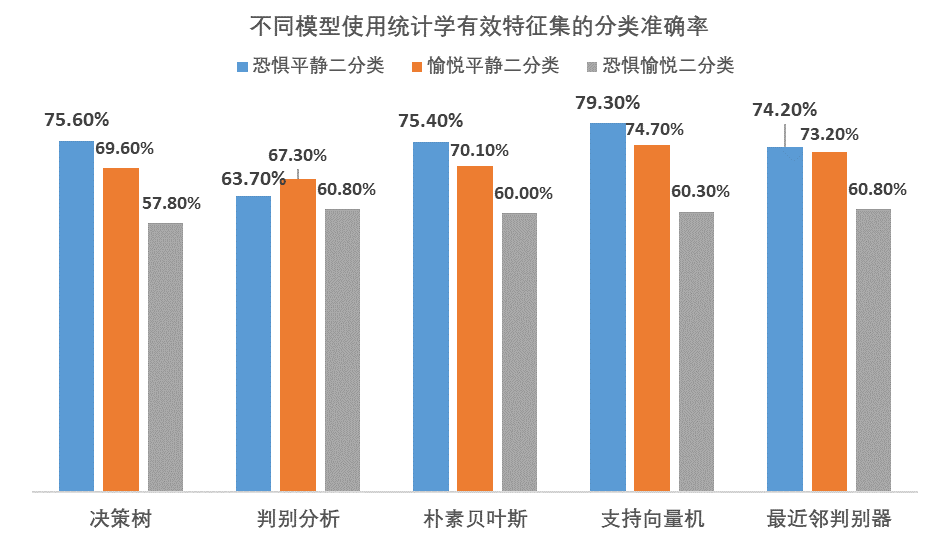
\includegraphics[width=.85\linewidth]{Model-Acurracy.png}
    \caption[不同模型使用统计学有效特征集的分类准确率]{不同模型使用统计学有效特征集的分类准确率}
    \label{fig:Model-Acurracy}
\end{figure}

分析\autoref{fig:Model-Acurracy}发现,五种机器学习模型中,支持向量机(SVM)相较其他分类器效果更好,最近邻判别器(KNN)次之。
进一步对比SVM和KNN的模型特点发现,KNN的相关模型是基于不同特征值之间的距离进行分类
(即如果一个样本在特征空间中的K个最相似样本大多属于某一个类别,则该样本也属于这个类别),在稀有事件的判别以及多分类问题上性能较好,但是其主要缺点在于计算量较大,尤其是在特征数较多时,
其惰性学习的特点会使得模型的内存开销、识别计算量都显著增加,进而导致预测效率的下降。
SVM的相关模型是基于训练集合在样本空间中找到一个“最大间隔”(两个异类支持向量到超平面的距离之和)的划分超平面进行分类,
其优势在于使用的样本量小而支持的样本空间维度高,具有良好的鲁棒性、寻优能力和泛化能力。

结合本研究的样本和特征特点,分类任务所使用的样本量较小而特征量及其中的非线性特征占比较大,与SVM的优势最为匹配,且主要聚焦情绪的二分类模型,未涉及SVM在多分类任务中的局限,所以选择SVM作为最终的模型构建方法。

在SVM核函数的选择方面,对比线性核、多项式核和高斯核三种SVM核函数在本研究的三个情绪二分类任务中的表现(\autoref{fig:SVM-Kurnal-Acurracy})后发现:线性SVM虽然计算速度较快但准确率、ROC曲线和混淆矩阵的表现相对较差;
二次、三次等多项式SVM和高斯SVM分类效果较好,但考虑到多项式核的过拟合现象更严重,同等分类效果下高斯核优势更大。在使用粗略高斯核、中等高斯核和精细高斯核的三种高斯SVM中,
中等高斯SVM的准确率、ROC曲线和混淆矩阵的表现较好,所以最终使用中等高斯SVM进行后续的分类任务,并采用5折交叉验证评估模型准确率。
\vspace{-1ex}
\begin{figure}[htbp]
    \centering
    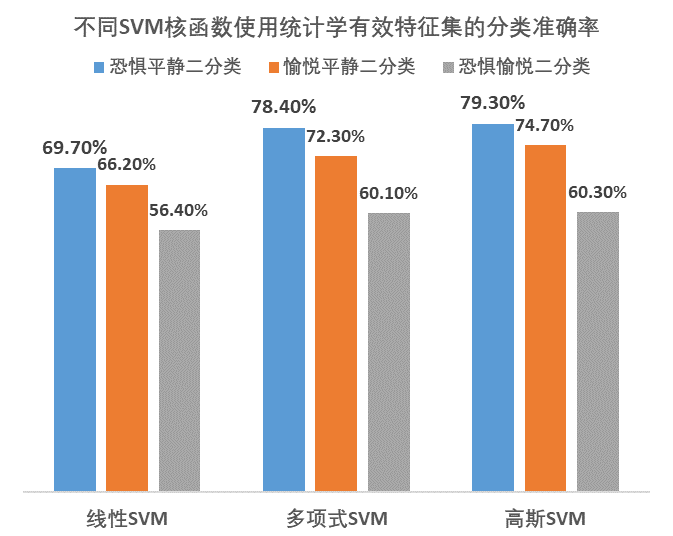
\includegraphics[width=.65\linewidth]{SVM-Kurnal-Acurracy.png}
    \caption[不同核函数使用统计学有效特征集的分类准确率]{不同核函数使用统计学有效特征集的分类准确率}
    \label{fig:SVM-Kurnal-Acurracy}
\end{figure}

\clearpage
\subsection{模型构建、优化与结果分析}

\subsubsection{分类模型构建与优化}

在机器学习模型的选择过程中,本研究将所有统计学有效特征作为输入,使用中等高斯SVM分别构建了恐惧平静二分类、愉悦平静二分类和恐惧愉悦二分类的初步分类模型,
但模型可能存在特征冗余、过拟合等问题,准确率等指标有待优化。为进一步降低各情绪分类模型的维度以减少模型训练时间和计算量并提高模型泛化能力,
本研究尝试通过特征组合的方式,选出各分类任务中特征量最少且分类效果最好的有效特征集。

考虑到本研究的样本数据不平衡(恐惧、愉悦和平静片段的比例大约为1:3:3),仅依据准确率不能全面地衡量模型性能和优化效果,
在准确率的基础上选择AUC值和混淆矩阵参数相关的精确率、召回率作为模型分类效果的评价指标。AUC值定义为ROC曲线与坐标轴所围面积,
取值范围一般为0.5$ \sim $1.0,且越接近1.0,说明分类模型效果越好;精确率(Precision)为被识别为正类别的样本中为正类别的比例,
召回率(Recall)为所有正类别样本中被正确识别为正类比的比例,公式定义如下:
\vspace{-1ex}
\begin{equation}
    \label{equ:Precision}
    Precision=\frac{TP}{TP+FP}
    \vspace{-4ex}
\end{equation}
\begin{equation}
    \label{equ:Recall}
    Recall=\frac{TP}{TP+FN}
    \vspace{1ex}
\end{equation}
$\qquad$其中:TP指真正类(即正确预测为正例的概率),FP指假正类(即错误预测为正例的概率),FN指假负类(即错误预测为负例的概率)。

现以恐惧平静二分类模型为例,说明本研究的模型优化过程(机器学习模型均为中等高斯SVM,以下不再赘述):

(1)使用统计学有效特征集初步构建情绪二分类模型:

将二分类任务的所有统计学有效特征作为输入,调整并最终确定使得模型分类效果最好的误分类代价矩阵为之后统一使用的参数(误分类代价矩阵即一个属于某类的实例被误分类为另一类的代价)。
如:将恐惧平静二分类任务中有14个统计学有效特征作为一个整体特征集输入,调整误分类代价矩阵中恐惧预测为平静的罚分为4.8时,模型的分类准确率、精确率、召回率和AUC值表现最好,则后续暂时统一使用4.8的罚分;

(2)寻找最优单特征模型:

使用调整好的误分类代价矩阵,将二分类任务的所有统计学有效特征逐个建立单特征分类模型,确定分类效果最优的单特征为最终分类模型特征集的首个特征。
如:将恐惧平静二分类任务中的14个统计学有效特征,每个特征单独作为输入,构建14个分类模型,比较后发现使用ECG\_corDim特征的模型分类效果最好,则确定该特征为恐惧平静分类模型特征集的首个特征;

(3)组合不同特征,寻找最优多特征模型:

在最优单特征的基础上加入其余效果较好的特征,寻找分类效果最好的最优双特征分类模型;在最优双特征的基础上再次加入其余效果较好的特征,寻找分类效果最好的最优三特征分类模型;以此类推,直至新增特征不能使得模型效果有明显提升,则新增特征前的最优特征集为初步确定的恐惧平静二分类任务的有效特征集。
如:将ECG\_corDim分别组合其余13个特征,发现ECG\_corDim + PPG\_K的特征组合分类效果最好,则PPG\_K确定为恐惧平静分类模型特征集的第二个特征,以此类推;

(4)模型参数调整,确定最优特征集:

对最优特征集构建的分类模型,再次调整误分类代价矩阵,若模型效果未能明显改善,则该最优特征集为恐惧平静二分类任务下的有效特征集;若模型效果得到进一步提升,则重新进行添加特征寻找最优特征集的操作步骤,直至确定最终的有效特征集。
如:恐惧平静二分类模型在ECG\_corDim + PPG\_K + RESP\_Gamma + PPG\_LF\_norm + RESP\_Delta + RESP\_PP\_std的六特征组合基础上,再增加特征均使得模型性能下降,所以不再增加特征。
最后调整误分类矩阵时发现,恐惧预测为平静的罚分调整为3.8时,模型的分类效果有小幅的优化,所以最终确定3.8的罚分+六特征组合为最优的恐惧平静二分类模型。

以下展示三个二分类任务中模型的具体优化过程(此处只展示各步骤中最优特征集的调整,其余特征因篇幅原因不做展示),恐惧平静二分类见\autoref{tab:Fear-Calm},愉悦平静二分类见\autoref{tab:Happy-Calm},恐惧愉悦二分类见\autoref{tab:Fear-Happy}。

\begin{table}[htbp]
    \centering
    \footnotesize
    \setlength{\abovecaptionskip}{0.1cm}
    \setlength{\belowcaptionskip}{0.2cm}
    \renewcommand\arraystretch{1.5}
    \caption[恐惧平静二分类模型优化过程。]{恐惧平静二分类模型优化过程}
    \label{tab:Fear-Calm}
    \setlength{\tabcolsep}{0.22cm}{
        \begin{tabular}{clccccl}
            \toprule
            \textbf{特征数} & \textbf{具体特征}          & \textbf{准确率} & \textbf{精确率} & \textbf{召回率} & \textbf{AUC值} & \textbf{备注}              \\ \midrule
            14              & \begin{tabular}[c]{@{}l@{}}恐惧平静二分类任务\\ 中的统计学有效特征\end{tabular}         & 79.30\%         & 80.40\%         & 79.00\%         & 0.88           & \begin{tabular}[c]{@{}l@{}}真实类(恐惧)预测为平静的\\ 代价设为4.8,后续不加说明则\\ 不作修改  \end{tabular} \\  \midrule
            1               & ECG\_corDim                & 23.70\%         & 100.0\%         & 50.00\%         & 0.68           &  \begin{tabular}[c]{@{}l@{}}准确率低是因为4.8的罚分使得\\ 恐惧被判错的代价过高,模型\\ 牺牲了平静被正确预测的概率 \end{tabular}                      \\ \midrule  
            2               & ECG\_corDim+PPG\_K         & 74.90\%         & 72.50\%         & 74.82\%         & 0.78           &                            \\ \midrule
            3               & \begin{tabular}[c]{@{}l@{}}ECG\_corDim+PPG\_K\\ +RESP\_Gamma\end{tabular} & 78.40\%         & 72.50\%         & 78.55\%         & 0.81           & \begin{tabular}[c]{@{}l@{}}平静被正确预测的概率比恐惧\\ 被正确预测的概率大很多,所\\ 以导致召回率偏高\end{tabular} \\ \midrule
            4               & \begin{tabular}[c]{@{}l@{}} ECG\_corDim+PPG\_K\\ +RESP\_Gamma+PPG\_LF\_norm\end{tabular} & 75.80\%         & 77.50\%         & 75.83\%         & 0.82           &                            \\ \midrule
            5               & \begin{tabular}[c]{@{}l@{}} ECG\_corDim+PPG\_K\\ +RESP\_Gamma+PPG\_LF\_norm+\\ RESP\_Delta\end{tabular} & 76.30\%         & 78.40\%         & 76.26\%         & 0.84           &                            \\ \midrule
            6               & \begin{tabular}[c]{@{}l@{}} ECG\_corDim+PPG\_K\\ +RESP\_Gamma+PPG\_LF\_norm+\\ RESP\_Delta+RESP\_PP\_std\end{tabular} & 78.60\%         & 84.30\%         & 78.42\%         & 0.88           & \begin{tabular}[c]{@{}l@{}}在此基础上继续添加特征反而\\ 降低了模型性能,调整误分类\\代价矩阵以优化模型\end{tabular} \\ \midrule
            6               & \begin{tabular}[c]{@{}l@{}} ECG\_corDim+PPG\_K\\ +RESP\_Gamma+PPG\_LF\_norm+\\ RESP\_Delta+RESP\_PP\_std\end{tabular} & 80.70\%         & 82.40\%         & 80.63\%         & 0.88           & \begin{tabular}[c]{@{}l@{}}代价调整为3.8效果最优,\\ 在此基础上继续添加特征均使\\ 得模型性能下降,因此确定该\\ 特征组合为最终的有效特征集\end{tabular} \\ \bottomrule
        \end{tabular}}
\end{table}

% 愉悦平静二分类如\autoref{tab:Happy-Calm}所示。
\begin{table}[h]
    \centering
    \footnotesize
    \setlength{\abovecaptionskip}{0.1cm}
    \setlength{\belowcaptionskip}{0.2cm}
    \renewcommand\arraystretch{1.35}
    \caption[愉悦平静二分类模型优化过程。]{愉悦平静二分类模型优化过程}
    \label{tab:Happy-Calm}
    \setlength{\tabcolsep}{0.22cm}{
        \begin{tabular}{clccccl}
            \toprule
            \textbf{特征数} & \textbf{具体特征}          & \textbf{准确率} & \textbf{精确率} & \textbf{召回率} & \textbf{AUC值} & \textbf{备注}              \\ \midrule
            23              & \begin{tabular}[c]{@{}l@{}}愉悦平静二分类任务\\ 中的统计学有效特征\end{tabular}         & 74.70\%         & 75.00\%         & 74.55\%         & 0.82           & \begin{tabular}[c]{@{}l@{}}愉悦预测为平静的代价设为1.4,\\ 后续不加说明则不作修改\end{tabular} \\ \midrule
            1               & ECG\_corDim                & 60.60\%         & 66.00\%         & 49.82\%         & 0.68           &                            \\ \midrule
            2               & ECG\_corDim+PPG\_SampEn    & 69.80\%         & 66.40\%         & 71.24\%         & 0.76           &                            \\ \midrule
            3               & \begin{tabular}[c]{@{}l@{}}ECG\_corDim+PPG\_SampEn\\ +ECG\_ApEn\end{tabular} & 72.70\%         & 67.30\%         & 75.36\%         & 0.80           &                            \\ \midrule
            4               & \begin{tabular}[c]{@{}l@{}}ECG\_corDim+PPG\_SampEn\\ +ECG\_ApEn+PPG\_Power\_ratio\end{tabular} & 73.90\%         & 69.40\%         & 76.26\%         & 0.81           & \begin{tabular}[c]{@{}l@{}}在此基础上继续添加特征但模\\ 型性能未改善,调整误分类代\\ 价矩阵以优化模型\end{tabular} \\ \midrule
            4               & \begin{tabular}[c]{@{}l@{}}ECG\_corDim+PPG\_SampEn\\ +ECG\_ApEn+PPG\_Power\_ratio\end{tabular} & 73.90\%         & 74.40\%         & 73.74\%         & 0.81           & \begin{tabular}[c]{@{}l@{}}代价调整为1.3,后续不加说明\\ 则不作修改\end{tabular} \\ \midrule
            5               & \begin{tabular}[c]{@{}l@{}}ECG\_corDim+PPG\_SampEn\\ +ECG\_ApEn+PPG\_Power\_ratio\\ +ECG\_K\end{tabular} & 75.00\%         & 74.70\%         & 75.15\%         & 0.82           & \begin{tabular}[c]{@{}l@{}}在此基础上继续添加特征均使\\ 得模型性能下降,因此确定该\\ 特征组合为最终的有效特征集\end{tabular} \\ \bottomrule
        \end{tabular}}
\end{table}
\vspace{-10ex}

% 恐惧愉悦二分类如\autoref{tab:Fear-Happy}所示。
\begin{table}[h]
    \centering
    \footnotesize
    \setlength{\abovecaptionskip}{0.1cm}
    \setlength{\belowcaptionskip}{0.2cm}
    \renewcommand\arraystretch{1.35}
    \caption[恐惧愉悦二分类模型优化过程。]{恐惧愉悦二分类模型优化过程}
    \label{tab:Fear-Happy}
    \setlength{\tabcolsep}{0.17cm}{
        \begin{tabular}{clccccccl}
            \toprule
            \textbf{特征数} & \textbf{具体特征}          & \textbf{准确率} & \textbf{\begin{tabular}[c]{@{}c@{}}精确率\\ (恐惧)\end{tabular}} & \textbf{\begin{tabular}[c]{@{}c@{}}召回率\\ (恐惧)\end{tabular}} & \textbf{\begin{tabular}[c]{@{}c@{}}精确率\\ (愉悦)\end{tabular}} & \textbf{\begin{tabular}[c]{@{}c@{}}召回率\\ (愉悦)\end{tabular}} & \textbf{AUC值} & \textbf{备注}              \\ \midrule
            13              & \begin{tabular}[c]{@{}l@{}}愉悦恐惧二分类任务\\ 中的统计学有效特征\end{tabular}         & 60.30\%         & 55.90\%                             & 59.34\%                             & 61.70\%                             & 58.32\%                             & 0.66           & \begin{tabular}[c]{@{}l@{}}恐惧预测为愉悦的代价为\\ 3.7,后续不说明则不修改\end{tabular} \\ \midrule
            1               & ECG\_NN\_mean              & 48.80\%         & 85.30\%                             & 57.60\%                             & 37.30\%                             & 71.30\%                             & 0.67           & \begin{tabular}[c]{@{}l@{}}愉悦被正确预测的概率\\ 比恐惧小很多,故恐惧\\ 精确率偏高\end{tabular} \\ \midrule
            2               & \begin{tabular}[c]{@{}l@{}}ECG\_NN\_mean\\ +RESP\_PP\_std  \end{tabular} & 56.10\%         & 78.40\%                             & 60.63\%                             & 49.10\%                             & 69.45\%                             & 0.68           &                            \\ \midrule
            3               & \begin{tabular}[c]{@{}l@{}}ECG\_NN\_mean\\ +RESP\_PP\_std\\ +ECG\_K\end{tabular} & 61.00\%         & 68.60\%                             & 62.36\%                             & 58.60\%                             & 65.11\%                             & 0.68           & \begin{tabular}[c]{@{}l@{}}继续添加特征反而使得模\\型性能下降,调整误分类\\ 代价矩阵以优化模型\end{tabular} \\ \midrule
            3               & \begin{tabular}[c]{@{}l@{}}ECG\_NN\_mean\\ +RESP\_PP\_std\\ +ECG\_K\end{tabular} & 62.60\%         & 63.70\%                             & 62.45\%                             & 63.70\%                             & 62.45\%                             & 0.68           & \begin{tabular}[c]{@{}l@{}}代价调整为3.6,后\\续不加说明则不作修改\end{tabular} \\ \midrule
            4               & \begin{tabular}[c]{@{}l@{}}ECG\_NN\_mean\\ +RESP\_PP\_std\\ +ECG\_K\\ +ECG\_WeEn\_threshold\end{tabular} & 63.40\%         & 64.70\%                             & 63.62\%                             & 61.70\%                             & 62.45\%                             & 0.67           & \begin{tabular}[c]{@{}l@{}}代价调整为3.5效果最\\ 优,在此基础上继续添\\ 加特征均使得模型性能\\ 下降,因此确定该特征\\ 组合为最终的有效特征集 \end{tabular} \\ \bottomrule
        \end{tabular}}
\end{table}

\clearpage
分析以上三表发现,恐惧平静二分类模型使用六特征集合实现了80.70\%的识别准确率、82.40\%的精确率、80.63\%的召回率和0.88的AUC值,
分类效果较好,且四个分类评价指标都超过了统计学有效特征集的分类效果,降维效果也较好。
愉悦平静二分类模型使用五特征集合实现了75.00\%的识别准确率、74.70\%的精确率、75.15\%的召回率和0.82的AUC值,分类效果较好,
虽然评价指标与模型优化前大致相同,但使用特征的数量从23降至5,实现了模型的有效降维。
恐惧愉悦二分类模型使用四特征集合实现了63.40\%的识别准确率、恐惧情绪64.70\%的精确率和63.62\%的召回率、愉悦情绪61.70\%的精确率和62.45\%的召回率以及0.67的AUC值,
分类效果相对一般,但分类效果对比模型优化前有了显著提升且降维效果也较好。

\subsubsection{结果分析}
进一步分析三个模型的分类效果发现:

(1) 从整体上看: 

通过特征组合寻找最优特征集的方式,能够在降低维度的同时实现与原统计学特征集相同甚至更优的分类效果,有效提升了模型的泛化能力。
这也说明部分特征虽然在统计学意义上具有显著性差异,但是其分布范围的重叠程度较大,在分类模型中效果较差。

在三个二分类模型中,恐惧平静二分类、愉悦平静二分类和恐惧愉悦二分类模型的准确率、精确率、召回率和AUC值依次下降,
恐惧愉悦二分类的分类效果相对较差。说明在这三种情绪状态中,恐惧和愉悦作为具有较高唤醒度的情绪,使得外周生理活动处于更加激活的状态,
与低唤醒度的平静状态能够较好区分;而恐惧和愉悦两种情绪之间虽然具有完全相反的效价,分属于消极和积极两类情绪,
但该指标可能更偏向于主观判断而在生理信号的改变上没有特别显著的表现,进而造成识别准确率的下降。
此外,恐惧愉悦二分类的识别效果不佳可能还与较高程度的愉悦情绪较难被诱发以及愉悦刺激材料的情绪唤起能力不足有关。

(2) 从单个分类模型来看: 

在恐惧平静二分类任务中,最终使用的有效特征包括心电信号的关联维数(非线性,P=0.036),脉搏波信号的K值(时域,P=0.000)和标准化低频能量(频域,P=0.000),
呼吸信号的PP间期序列标准差和一阶及二阶差分绝对值的均值(均为时域,P值分别为0.000、0.032和0.036)。时域特征占比相对较大。

在愉悦平静二分类任务中,最终使用的有效特征包括心电信号的关联维数和近似熵(均为非线性,P值均为0.000)、K值(时域,P=0.000),脉搏波信号的低高频能量比(频域,P=0.000)和样本熵(非线性,P=0.000)。
非线性特征占比大且有效特征全部是统计学分析中差异最为显著的部分特征。

在恐惧愉悦二分类任务中,最终使用的有效特征包括心电信号的RR间期均值和K值(均为时域,P值分别为0.000和0.002)、小波熵(非线性,P=0.025),呼吸信号的PP间期序列标准差(时域,P=0.000)。
时域特征占比较大且有效特征几乎都是统计学分析中差异最为显著的部分特征。

(3) 从单个生理信号来看: 

心电信号相关的特征在三个分类模型中都最为有效,表明心电对于情绪状态的区分贡献度较大。然而不同维度上的心电特征,分类效果差异很大,
恐惧平静二分类和愉悦平静二分类模型中全部使用的是心电信号的非线性特征而恐惧愉悦二分类任务中使用的全部是时域特征,
表明心电信号的复杂程度在情绪发生时会有较为显著的改变,而恐惧和愉悦情绪之间的变化更多地反映在心电的波形特征中,这与统计学分析的结果也保持一致。

脉搏波相关的特征由于在恐惧愉悦二分类任务中不具有统计学上的显著性差异,所只在恐惧平静二分类和愉悦平静二分类模型中使用,同时所使用的特征以频域为主,这与统计学分析的结果也保持一致。 

呼吸信号相关的特征在恐惧平静二分类和恐惧愉悦二分类模型中起到重要的辅助作用,而在愉悦平静二分类模型中效果不佳,表明呼吸信号对于恐惧情绪的发生更为敏感,这与统计学分析的结果也保持一致。 

(4) 从单个特征来看: 

一些特征在多个二分类模型中都有效,如心电信号的关联维数在恐惧平静二分类和愉悦平静二分类模型中都是分类效果最好的特征,呼吸信号的PP间期标准差在恐惧平静二分类和恐惧愉悦二分类中起到重要的辅助作用,心电信号的K值在愉悦平静二分类和恐惧愉悦二分类模型中提供了较好的优化效果,表明这些特征对于情绪状态的变化更为敏感,在情绪识别研究中可能更加有效。




\clearpage
\section{总结与展望}

\subsection{总结}
本研究旨在提供一种简便、合理、有效的情绪识别方案,构建多信号、多维度、多参数的情绪识别模型。研究内容主要包括以下几个方面: 

(1)情绪诱发材料的筛选与生理信号的采集: 

设计并完成了情绪刺激材料评价实验(66名被试),运用成功指数和唤醒度效价检验,筛选出能够有效诱发恐惧、愉悦、平静三种情绪且具有普适性的视频材料。在此基础上完成了情绪诱发生理实验(66名被试,与情绪刺激材料评价实验不重复),在成功唤起被试目标情绪的同时采集心电、脉搏和呼吸信号,用于后续情绪特征集的构建。

本研究中视频材料的筛选、情绪诱发及数据采集的流程由自主设计的Python程序进行控制,
心电、脉搏和呼吸信号由迈瑞ePM 12M生理参数监护仪(医疗级别)进行采集,
两者共同构建了一种相对简便、规范和可推广的情绪识别实验流程。
对于恐惧、愉悦和平静外的其他基础情绪或复合情绪(如愤怒、悲伤等),均可以在简单替换刺激材料后直接使用相同程序和设备以相同流程进行实验和研究,
有利于更深入和全面地进行情绪识别研究。

(2)情绪特征的提取与特征的统计学分析: 

针对情绪诱发生理实验采集到的三种外周生理信号,通过数据清洗、信号预处理和特征提取操作,从时域、频域、非线性三个维度共提取80个特征,构成多信号多维度多参数的情绪特征集。

然后通过非参数检验的统计学方法,分析特征集在各分类任务中的显著性,最终筛选出14、23和13个在恐惧平静二分类、愉悦平静二分类和恐惧愉悦二分类任务中有显著差异的统计学有效特征,用于后续机器学习模型的构建与优化。

同时,对统计学有效特征的维度分布,与生理变化的内在联系做出分析,发现在恐惧和愉悦状态下,生理信号的复杂度会发生较为显著的变化,同时交感神经系统、副交感神经系统以及两者的均衡性或平衡性也会发生改变,具体反映到生理信号各频段功率及其比值特征的变化中。这些信息有利于后续进一步研究生理信号与不同情绪之间的特异性关联。

(3) 情绪分类模型的构建、优化与结果分析: 

使用中等高斯SVM构建情绪分类模型应用于恐惧平静二分类、愉悦平静二分类和恐惧愉悦平静二分类,并通过特征组合的方式,选出各分类任务中特征量最少且分类效果最好的有效特征集。最终,恐惧平静二分类模型使用六特征集合实现了80.70\%的识别准确率,愉悦平静二分类模型使用五特征集合实现了75.00\%的识别准确率,恐惧愉悦二分类模型使用四特征集合实现了63.40\%的识别准确率,分类效果与使用统计学有效特征集的分类模型相比有所改善且模型维度大大降低,有效提升了模型的泛化能力。


\subsection{展望}

论文基于外周生理信号进行情绪识别的研究,取得了一些成果,但还存在以下一些不完善之处:

(1)情绪诱发实验的改进

论文只研究了恐惧、愉悦和平静三种情绪状态,主要完成了三种情绪之间的二分类任务。但情绪的类别远不止这三种情绪,今后可选择其他的基本情绪以及复合情绪(如悲伤、愤怒等)进行研究,以适应更多的应用场景。

同时,本研究的被试对象均为浙江大学的在校学生,样本较为集中,缺乏对不同地区、不同年龄段、不同职业等被试的研究,缺乏对地区、年龄、职业等因素与情绪诱发效果之间的关系的关注,也未验证所得情绪分类模型在其他各类群体中的适用性及可推广性。今后可以增加不同地区、不同年龄、不同职业的被试样本,以构建对于各类群体均有效的情绪识别模型。

(2)数据分析过程的改进

本研究只使用了心电、脉搏和呼吸三种外周生理信号,没有使用其他一些与情绪变化有特异性关联的生理信号(如肌电、皮肤电、眼电等),所提取到的情绪特征集有很大的扩充空间。今后可以融合更多的生理信号,探究各种生理变化与情绪的内在关联,建立更加全面的多维度情绪生理特征集。
同时也可结合目前已经较为完备的(通过面部表情、身体姿态和语音信息等进行情绪识别的方法),辅助验证生理信号构建一种多模态特征集。

在数据处理方面,因为已经通过情绪刺激材料评价实验筛选出能够有效诱发恐惧、愉悦、平静三种情绪且具有普适性的视频片段,本研究直接对情绪生理唤醒实验的被试数据进行20s的分段,没有充分利用被试的主观评价,忽略了情绪诱发强度对生理信号的影响。今后可以依据主观评价为特征赋权重,或将其作为特征变化的验证指标,更全面和深入地探究生理信号与情绪之间的关联。
同时,本研究只选用了三个信号都有效的被试数据,两个信号有效的被试数据未被采用,其实可以对这部分数据只进行两个有效信号的处理,这样能够获得更多的情绪片段。

(3)情绪识别模型的优化

本研究使用中等高斯SVM构建情绪分类模型并通过特征组合的方式进行优化,取得了不错的分类和降维效果,但优化过程是通过人工选择进行,工作量很大且不易推广,今后可以尝试如过滤法(Filter)、包装法(Wrapper)、嵌入法(Embedded)等更多的特征选择和降维方法,以更好地筛选最优特征集。

% 此外,由于情绪相关的生理变化个体差异性较大,不同被试间的相同情绪状态可能存在不同的变化趋势,对于同一刺激材料的情绪反应也可能大不相同。因此试图使用所有被试数据构建统一的识别模型的思路存在很多阻碍。但在某些特殊的应用领域(如对航天员情绪的识别和追踪,人数少而识别准确率要求高),可以单独构建每个个体的情绪识别模型。这样虽然牺牲了模型的可推广性和应用范围,但可以显著提升识别效果,也极具实际意义。
